\documentclass[lettersize,journal]{IEEEtran}
\usepackage{amsmath,amsfonts}
\usepackage{algorithmic}
\usepackage{algorithm}
\usepackage{array}
\usepackage[caption=false,font=normalsize,labelfont=sf,textfont=sf]{subfig}
\usepackage{textcomp}
\usepackage{stfloats}
\usepackage{url}
\usepackage{verbatim}
\usepackage{graphicx}
\usepackage{cite}
\usepackage{booktabs}
\usepackage{multirow}
\usepackage{tabularx}
\usepackage{threeparttable}
\usepackage{balance}
\usepackage{xcolor}
\usepackage{microtype}
\usepackage{siunitx}
\usepackage{placeins}
\usepackage{hyperref}
\hypersetup{hidelinks}
\graphicspath{{figures/}}
\sisetup{detect-all}
\hyphenation{op-tical net-works semi-conduc-tor IEEE-Xplore}

\begin{document}

\title{Auditing Set-of-Vision Prompting for Zero-Shot Emotion Recognition: Accuracy and Demographic Robustness in Two Open Vision-Language Models}

\author{Thammandra~Saketh~Ram, Veeramallu~Varun~Babu, and Yellampati~Lukesh\\\href{https://github.com/varunbabuvb/ml_project}{Project repository: github.com/varunbabuvb/ml\_project}}

\maketitle

\begin{abstract}
Visual prompting is intended to make vision-language models attend to and reason about selected image regions. Set-of-Vision (SoV) prompting uses bounding boxes, numbered face markers, and facial landmarks to support face localization and expression classification. This report presents an empirical audit of an implementation of SoV prompting on the Expression in-the-Wild (ExpW) dataset. We evaluate a primary LLaVA-1.5-7B model and a second-model check using Qwen2.5-VL-7B-Instruct. The evaluation compares plain inputs with cumulative visual conditions that add boxes, numbering, and landmark dots. We assess single-face context crops, multi-face images, and performance across FairFace-estimated demographic groups. Balanced accuracy is the principal single-face metric, with paired image-level bootstrap intervals used for uncertainty estimation. In the single-face core set, raw balanced accuracy decreased under SoV relative to Plain for both models: by 5.4 percentage points for LLaVA and 8.1 points for Qwen. After self-calibration, the LLaVA difference was smaller and its interval included zero, whereas the Qwen reduction remained. The multi-face results also depend on whether the comparison changes both the overlay and the prompt or holds the prompt fixed. No race-group or gender difference in the SoV effect was detected in the core analysis, although the intervals do not establish equivalence. These findings are specific to the evaluated models, dataset, crops, prompts, and implementation; they do not establish that visual prompting is generally ineffective.
\end{abstract}

\begin{IEEEkeywords}
Vision-language models, visual prompting, facial expression classification, demographic robustness, balanced accuracy, Set-of-Vision.
\end{IEEEkeywords}

\section{Introduction}
Vision-language models (VLMs) accept visual inputs together with natural-language instructions and can perform a range of zero-shot recognition tasks. Their flexibility makes them attractive for facial-expression classification, where a model must interpret local facial appearance while retaining enough context to distinguish the target face from other people and objects in the image. However, a natural-language instruction alone may not make the intended face sufficiently salient, particularly in group photographs.

Visual prompting attempts to guide a model by modifying the image itself. Instead of relying only on a textual reference such as ``the person on the left'', visual prompts add graphical markers that indicate relevant regions. Set-of-Vision (SoV) prompting applies this idea to facial-expression recognition by progressively adding face bounding boxes, numbered identifiers, and facial landmarks. The original SoV work reports improvements in emotion recognition and face-related tasks using these visual cues \cite{zhang2024sov}. The present project audits whether a similar strategy improves expression classification in a separate experimental setup.

The term \emph{emotion recognition} is used here in the conventional machine-learning sense of predicting a dataset-assigned facial-expression category. The predicted category is not a direct measurement of a person's internal emotional state. This distinction is important because facial appearance, annotator labels, and subjective emotional experience are not interchangeable.

Our study focuses on two questions. First, does adding SoV-style visual information improve the balanced accuracy of zero-shot expression classification on ExpW context crops? Second, does the effect vary across demographic groups estimated by a separate face-attribute model? We also examine multi-face images, where target-face reference and prompt wording interact, and conduct a shuffled-tag probe to test whether models can read the numeric identifiers placed on faces.

The primary model is LLaVA-1.5-7B. Qwen2.5-VL-7B-Instruct is used as a second-model check, not as a basis for ranking the models. The two models exhibit substantially different Neutral-label behaviour and were not subjected to identical development-set selection procedures. Accordingly, all main findings are interpreted per model.

The central result is that, under this experimental setup, SoV did not improve balanced accuracy. Raw performance was lower under SoV for both models. After answer-bias correction, the LLaVA reduction became small and its interval included zero, while the Qwen reduction persisted. The report also distinguishes comparisons in which overlay and prompt change together from comparisons that hold the prompt fixed. This distinction is essential for interpreting the multi-face experiments.

The contributions of this project are an implemented SoV-style evaluation pipeline, paired comparisons of cumulative visual conditions, an analysis of estimated demographic-group robustness, a half-size landmark ablation, a multi-face prompt/overlay comparison, and a shuffled-tag reading probe.

\section{Related Work}
\subsection{Visual prompting and Set-of-Vision}
Visual prompting modifies an image with graphical cues to direct a vision-language model toward a region or object. Examples include boxes, circles, and other visual markers that supplement a natural-language instruction. SoV applies a staged combination of bounding boxes, numbered face identifiers, and facial landmarks to facial-expression recognition. Its motivation is that boxes identify face regions, numbers distinguish multiple faces, and landmarks provide additional spatial information about facial structure \cite{zhang2024sov}.

The present work follows the same broad progression but should be understood as an implementation and audit of the method, not as a claim of exact reproduction of every implementation detail in the original paper. In particular, the visual conditions used here are cumulative: Plain, Box, Box+Number, and SoV. Consequently, the landmark comparison estimates the effect of adding landmark dots to an already boxed and numbered image. It is not a factorial test of landmark dots in isolation.

\subsection{Vision-language models}
LLaVA connects a visual encoder to a language model and is trained for visual instruction following \cite{liu2023llava,liu2024llava15}. LLaVA-1.5 strengthens this baseline using a CLIP vision encoder and visual instruction-tuning data. Qwen2.5-VL is a later vision-language model family with a visual processing design that supports dynamic-resolution inputs \cite{bai2025qwen25vl}. These model families differ in their visual encoders, image processing, tokenization, and language-model behaviour. A nominal crop size of 336 by 336 pixels therefore does not imply identical internal visual representations.

\subsection{Face attributes and demographic robustness}
FairFace was introduced as a face-attribute dataset designed to provide more balanced race representation and labels for race, gender, and age \cite{karkkainen2021fairface}. In this project, FairFace is used as an estimator of demographic attributes for ExpW faces. These outputs are model estimates, not self-reported identity or ground-truth demographic labels. The estimates are filtered for stability across two crop paddings before being used in subgroup analyses.

The demographic analysis is therefore an audit across operational groups produced by a face-attribute model. It does not establish cultural identity, nationality, ethnicity in a sociological sense, or cross-cultural generalization. We avoid the term ``cross-cultural'' because the evaluated data do not contain verified cultural or geographic labels.

\subsection{In-the-wild expression datasets}
ExpW contains 91,793 face images with seven expression categories: Angry, Disgust, Fear, Happy, Sad, Surprise, and Neutral \cite{peng2016expw}. Its in-the-wild imagery provides variation in pose, illumination, and background, but the annotations are not noise-free. The present evaluation uses a filtered subset of ExpW and treats its expression labels as annotator-assigned targets. RAF-DB was considered in the initial project plan but was not used in the final experiments because dataset access was not obtained.

\section{Problem Formulation and Research Questions}
Let $x_i$ denote a context crop for target face $i$, $y_i \in \mathcal{Y}$ its ExpW expression label, and $c$ a visual condition. The model receives an image-prompt pair and produces scores over the seven candidate labels. The evaluation asks whether changing $c$ changes the correctness of the predicted label and whether the effect differs across estimated demographic groups.

The research questions are:
\begin{itemize}
    \item \textbf{RQ1:} Does SoV-style prompting improve single-face balanced accuracy relative to a Plain visual input?
    \item \textbf{RQ2:} What is the incremental effect of adding boxes, numbers, and landmark dots in the cumulative condition sequence?
    \item \textbf{RQ3:} Does the SoV--Plain performance difference vary across FairFace-estimated race groups or gender groups? Age-group results are treated as exploratory.
    \item \textbf{RQ4:} In multi-face images, how do visual overlays and target-reference prompts affect per-face classification? What changes when the prompt is held fixed?
    \item \textbf{RQ5:} Which patterns are consistent across LLaVA and Qwen? Direct cross-model contrasts are post hoc.
\end{itemize}

\section{Methodology}
\subsection{Experimental pipeline}
Fig.~\ref{fig:pipeline} presents the eight-stage experimental architecture supplied by the project team. ExpW provides the images and expression annotations. Face processing produces detections and landmarks, followed by target-face matching. Context crops are then prepared and rendered under the visual-prompt conditions. LLaVA and Qwen process the resulting image-prompt inputs. Candidate-label scores are converted into predictions, and the outputs are analysed using balanced accuracy, bootstrap intervals, demographic subgroups, and additional multi-face and tag-reading experiments.

\begin{figure*}[!t]
\centering
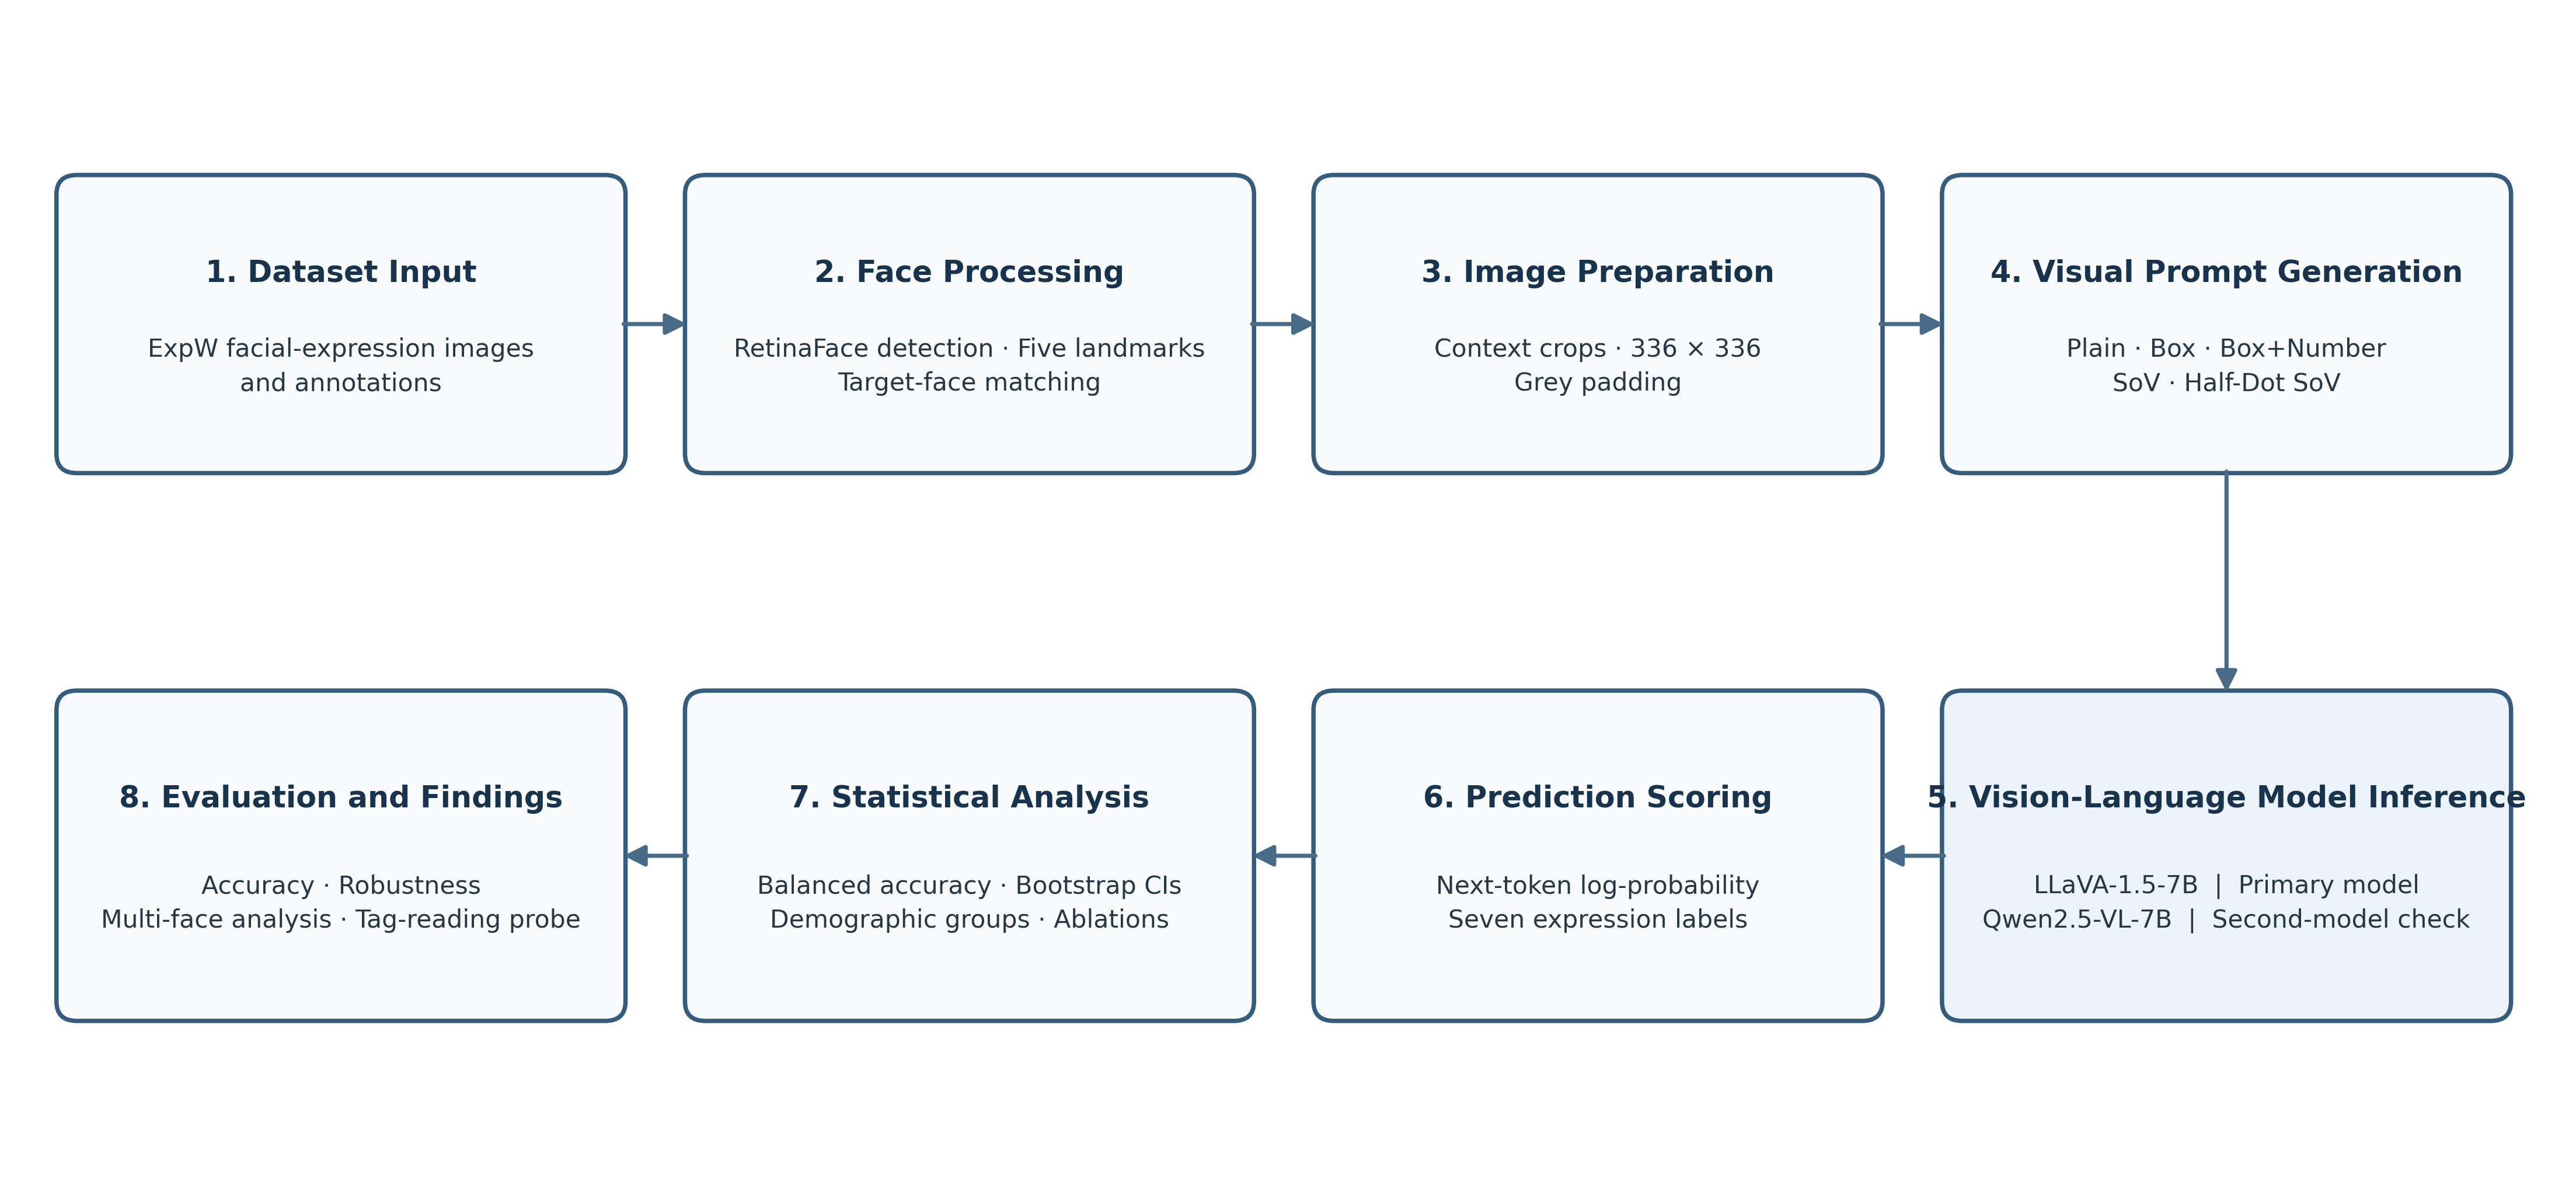
\includegraphics[width=0.96\textwidth]{project_architecture.png}
\caption{Eight-stage experimental pipeline for the SoV audit. The FairFace demographic-estimation branch supplies estimated group labels for the statistical analysis; it is not part of the emotion-classification inference path.}
\label{fig:pipeline}
\end{figure*}

\subsection{Face detection, landmarks, and matching}
RetinaFace is used for face detection and five-point facial landmark localization \cite{deng2020retinaface}. The five landmarks correspond to the eye, nose, and mouth reference points used by the overlay pipeline. The implementation applies overlap handling to detections and assigns left-to-right identifiers for numbered conditions. Target ExpW faces are matched to detected faces using one-to-one matching with an intersection-over-union threshold of 0.3. This matching step links the annotated target face to the corresponding detected face used to construct the visual prompt.

\subsection{Context-crop preparation}
The evaluated input is a face-centred context crop, not the complete original image. The crop is constructed using a scale based on 2.75 times the larger side of the target face box, then made square with grey padding and resized to 336 by 336 pixels. Retaining context around the face is intended to preserve nearby scene information while ensuring that the target face remains prominent. The same nominal output dimensions do not guarantee identical internal processing by the two VLMs; Qwen2.5-VL supports dynamic-resolution visual processing, and the models have different visual tokenization paths.

\subsection{Visual conditions}
The core conditions form a cumulative sequence:
\begin{enumerate}
    \item \textbf{Plain:} no face overlay.
    \item \textbf{Box:} bounding-box marking of detected faces.
    \item \textbf{Box+Number:} bounding boxes with numeric identifiers.
    \item \textbf{SoV:} boxes, numbers, and facial landmark dots.
    \item \textbf{Half-dot SoV:} the SoV condition with reduced landmark-dot size.
\end{enumerate}
The half-dot condition is an announced ablation added after the initial core results. It is not a separate factorial component. Because the design is cumulative, the comparison SoV minus Box+Number measures the effect of adding dots to the boxed-and-numbered condition. It cannot isolate a dots-only effect or estimate interactions among independently varied components.

\subsection{Model inference and candidate-label scoring}
The primary model is LLaVA-1.5-7B. Qwen2.5-VL-7B-Instruct is evaluated as a second-model check. Both are run in 4-bit quantized configurations on a Colab T4 GPU; Qwen is reported as using float16 computation with 4-bit weights. The recorded model identifiers are LLaVA-1.5-7B (llava-hf/llava-1.5-7b-hf) and Qwen2.5-VL-7B-Instruct (Qwen/Qwen2.5-VL-7B-Instruct).

The scoring implementation uses a single forward pass and obtains next-token log-probability scores for the seven candidate expression labels. The candidate set is Angry, Disgust, Fear, Happy, Sad, Surprise, and Neutral. The highest-scoring candidate is used as the predicted label. The seven candidate-label scores are normalized over the candidate set for prediction. The logged probability-mass diagnostic is reported in the Experimental Setup section.

\subsection{Demographic estimation}
FairFace predictions are generated from two crop paddings. Race, gender, and age estimates are retained or grouped according to the project's stability rule. The two-crop agreement reported by the project summary is 75.7\% for race, 95.0\% for gender, and 73.5\% for age. These values measure agreement between two crop settings, not accuracy against verified identity labels.

The race groups used in the analysis are operational categories labelled Caucasian-like, Asian, and Black. Gender and age categories are used only where the stability criterion is satisfied. Indian and Latino estimates are not separately represented in the final three-group race analysis. Group labels are interpreted as model-estimated attributes rather than definitive descriptions of the people pictured.

\subsection{Multi-face experiment and comparison definitions}
The multi-face experiment contains images with multiple target faces. The prompt may refer to a target by its position (for example, a positional or centre-based reference) or by a numeric identifier. The overlay and prompt are not always paired identically across all arms. We therefore distinguish two comparison types throughout the report:
\begin{itemize}
    \item \textbf{As-designed comparison:} the overlay and the associated prompt may both change between conditions. This comparison describes the full experimental arm as implemented.
    \item \textbf{Matched-prompt comparison:} the prompt is held fixed while the overlay changes. This comparison more directly estimates the effect of the overlay manipulation.
\end{itemize}
The matched-prompt arms are available for the 997 faces in mixed images. Mechanism-level interpretation is based on matched-prompt contrasts, not on as-designed contrasts that change both overlay and prompt. The multi-face set contains 2,818 target faces, of which 2,816 have scored outputs, across 1,250 images. 

\subsection{Shuffled-tag reading probe}
A separate probe tests whether the models read numeric tags rather than infer a face's identifier from its left-to-right position. The tag numbers are shuffled so that the number displayed on a face does not correspond to its ordinal position. The model is asked to report the tag associated with the leftmost or rightmost face. Chance-level exact matching is approximately 23\% under the probe's tag distribution. Above-chance performance indicates tag-reading consistency on this probe; it does not establish that reading the tags caused any downstream classification improvement.

\section{Experimental Setup}
\subsection{Dataset and evaluated subsets}
ExpW contains 91,793 annotated face images in its full release. The project pipeline reports duplicate removal and filtering before constructing the evaluation subsets. The core single-face set contains 1,473 target faces from 1,461 images. A development set of 280 images is described as image-disjoint from the core set, with seed 42. The multi-face evaluation contains 1,250 images and 2,818 target faces; 2,816 targets have model outputs. Of the multi-face images, 428 are mixed images containing 998 target faces. The counts below describe the evaluated subsets used in the reported analyses.

\begin{table}[!t]
\caption{Current dataset and evaluation-set counts.}
\label{tab:dataset}
\centering
\footnotesize
\begin{tabular}{lrr}
\toprule
Subset & Images & Target faces \\
\midrule
Development & 280 & -- \\
Single-face core & 1,461 & 1,473 \\
Multi-face evaluation & 1,250 & 2,816 scored \\
Mixed multi-face subset & 428 & 998 \\
\bottomrule
\end{tabular}
\end{table}

\subsection{Models and runtime}
LLaVA-1.5-7B is the primary model and was subjected to development-set gating. Qwen2.5-VL-7B-Instruct is the second-model check and was not dev-gated; no Qwen dev-calibrated variant is available. Both model families are evaluated using quantized weights. Both models were run with 4-bit quantised weights on Colab T4 GPUs; Qwen used float16 computation. Qwen was not dev-gated, and no Qwen development-calibrated result is reported.

\subsection{Metrics and class sets}
Balanced accuracy is used as the primary single-face metric because it gives equal weight to each evaluated class rather than allowing common labels to dominate the aggregate. For $K$ classes, balanced accuracy is
\begin{equation}
\mathrm{BA} = \frac{1}{K}\sum_{k=1}^{K}\frac{\mathrm{TP}_k}{\mathrm{TP}_k+\mathrm{FN}_k}.
\end{equation}
The principal result uses all seven expression labels. Additional analyses omit Neutral or use restricted class sets where specified in the analysis outputs. Multi-face results report per-face accuracy for all target faces and a separate ``other-emotion'' subset comprising Angry, Disgust, Fear, Sad, and Surprise. The latter subset contains 301 faces. It is not described as ``expressive faces'', because Happy is also an expression category.

\subsection{Uncertainty and evidence hierarchy}
Paired differences are reported in percentage points (pp), with the sign defined as condition A minus condition B. The 95\% intervals are percentile bootstrap intervals over images, using 2,000 resamples and seed 42. Images, rather than individual faces, are the resampling unit so that faces from the same image remain clustered.

The evidence labels used in the report are:
\begin{itemize}
    \item \textbf{[pre]}: analysis rule or contrast fixed before the results were inspected.
    \item \textbf{[ann]}: analysis announced before its run but selected after initial core results; the half-dot ablation belongs here.
    \item \textbf{[post hoc]}: analysis selected after seeing results, including direct cross-model contrasts and several subgroup explorations.
\end{itemize}
The primary contrast is SoV minus Plain, raw balanced accuracy, all seven classes, on the core set, separately for each model. Component contrasts and calibration analyses are secondary. Age-band and detailed subgroup patterns, as well as direct cross-model differences, are exploratory or post hoc. An interval excluding zero is described as a detected difference under this analysis; an interval including zero is described as not detected. Failure to detect a difference is not evidence of equivalence, particularly because no equivalence margin was specified.

\subsection{Development-set selection and calibration}
LLaVA was gated using the development set. The project notes report a Plain macro-F1 of 0.361 against a pre-set threshold of 0.25, and a prompt comparison of 0.323 versus 0.310. Qwen was not subjected to the same gate. Both models have raw and self-calibrated analyses; only LLaVA has a development-calibrated variant. ``Answer-bias correction'' refers specifically to the project's self-calibrated scoring variant and should not be interpreted as a general correction of all model biases.

\subsection{Scoring validity}
The result files contain a probability-mass field and an error field for every recorded job. Table~\ref{tab:scoringvalidity} summarizes these diagnostics by condition. The reported means are calculated over all logged records for each condition; Box+Number and SoV include additional prompt-query records beyond the 1,473-face paired core subset.

\begin{table*}[!t]
\caption{Scoring diagnostics from the core result JSONL files. Mean mass is the average probability mass assigned to the seven candidate labels. Error counts are recorded inference/scoring errors.}
\label{tab:scoringvalidity}
\centering
\footnotesize
\begin{tabular}{llrrr}
\toprule
Model & Condition & Logged records & Mean candidate mass & Errors \\
\midrule
LLaVA & Plain & 1,473 & 0.9867 & 0 \\
LLaVA & Box & 1,473 & 0.9858 & 0 \\
LLaVA & Box+Number & 1,741 & 0.9856 & 0 \\
LLaVA & SoV & 1,741 & 0.9857 & 0 \\
Qwen & Plain & 1,473 & 0.9921 & 0 \\
Qwen & Box & 1,473 & 0.9925 & 0 \\
Qwen & Box+Number & 1,741 & 0.9932 & 0 \\
Qwen & SoV & 1,741 & 0.9905 & 0 \\
\bottomrule
\end{tabular}
\end{table*}


\section{Results}
\subsection{Single-face core: overall performance}
Table~\ref{tab:core} presents the raw balanced accuracy for the four principal conditions. Plain is the reference condition. In both models, Box and Box+Number remain close to Plain, while SoV has lower balanced accuracy.

\begin{table*}[!t]
\caption{Single-face core balanced accuracy, all seven classes. Bracketed values are 95\% image-cluster bootstrap intervals.}
\label{tab:core}
\centering
\footnotesize
\begin{tabular}{lcc}
\toprule
Condition & LLaVA-1.5-7B & Qwen2.5-VL-7B-Instruct \\
\midrule
Plain & 0.428 [0.410, 0.447] & 0.493 [0.473, 0.515] \\
Box & 0.419 [0.401, 0.438] & 0.492 [0.472, 0.512] \\
Box+Number & 0.417 [0.398, 0.435] & 0.498 [0.477, 0.519] \\
SoV & 0.374 [0.355, 0.394] & 0.412 [0.393, 0.432] \\
\bottomrule
\end{tabular}
\end{table*}

\begin{figure}[!t]
\centering
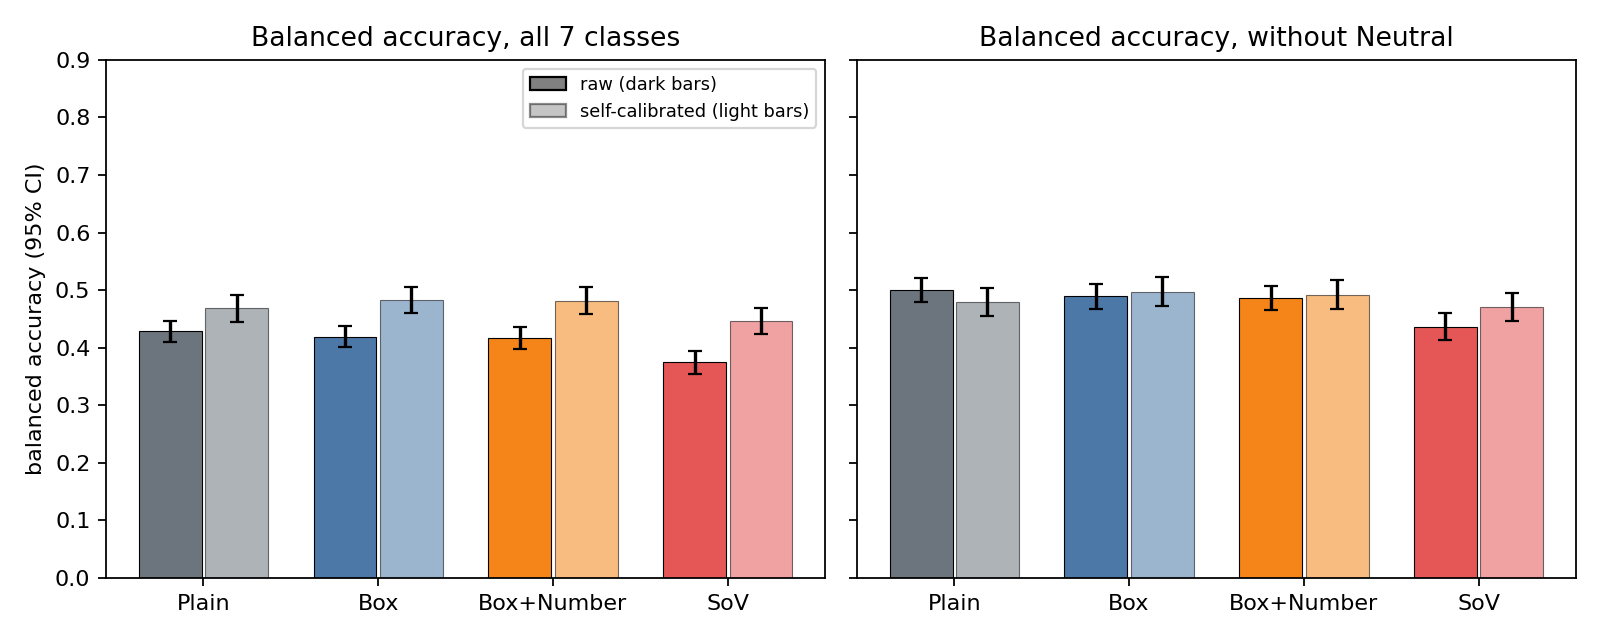
\includegraphics[width=\columnwidth]{core_llava_overall.png}
\caption{LLaVA single-face core balanced accuracy by visual condition.}
\label{fig:corellava}
\end{figure}
\begin{figure}[!t]
\centering
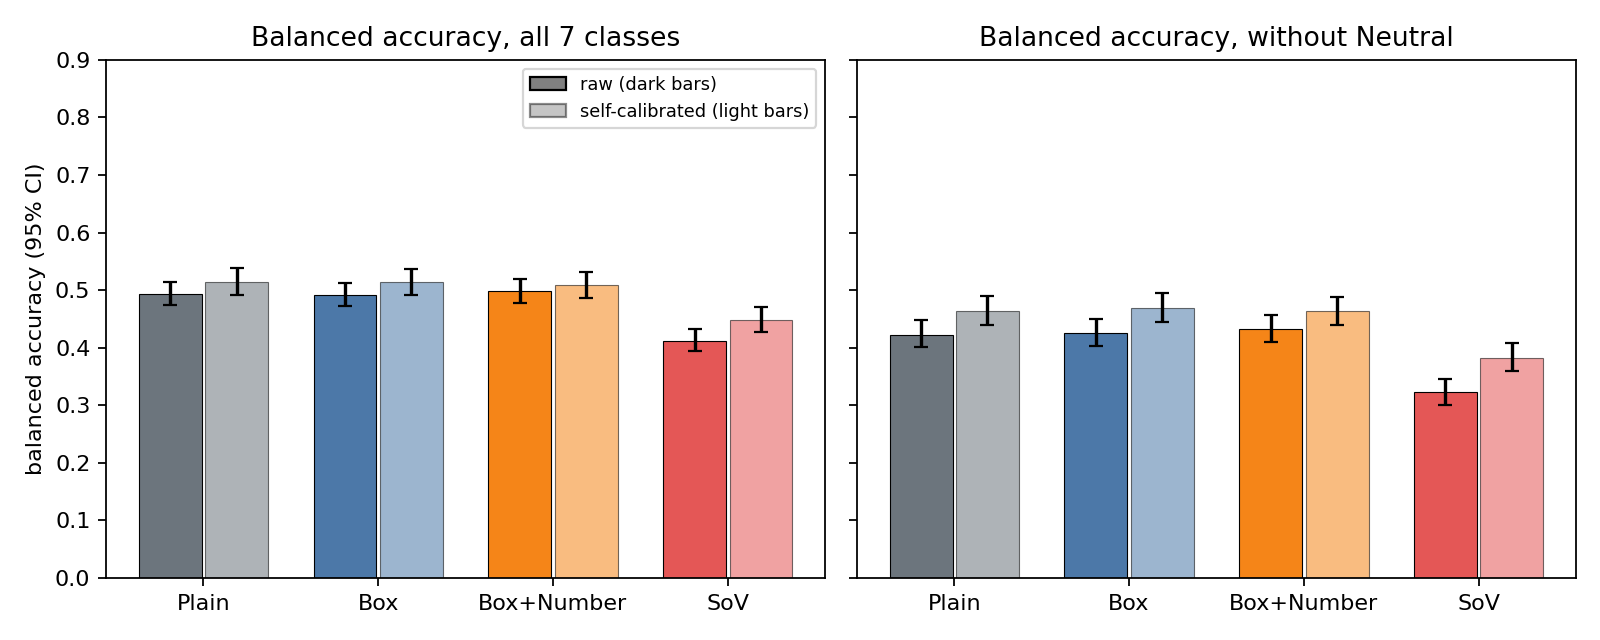
\includegraphics[width=\columnwidth]{core_qwen_overall.png}
\caption{Qwen single-face core balanced accuracy by visual condition.}
\label{fig:coreqwen}
\end{figure}

The paired SoV--Plain difference is $-5.4$ pp for LLaVA (95\% CI: $[-7.3,-3.5]$) and $-8.1$ pp for Qwen (95\% CI: $[-10.0,-6.2]$). The Box--Plain differences are $-0.9$ pp ([$-2.0,+0.2$]) and $-0.2$ pp ([$-1.6,+1.2$]), respectively. Box+Number--Plain is $-1.2$ pp ([$-2.3,+0.0$]) for LLaVA and $+0.5$ pp ([$-1.0,+1.8$]) for Qwen. These results do not show a balanced-accuracy benefit from the visual conditions tested.

\subsection{Component contrasts and the cumulative design}
The SoV--Box+Number contrast is $-4.2$ pp ([$-6.0,-2.4$]) for LLaVA and $-8.5$ pp ([$-10.5,-6.6$]) for Qwen. This is the comparison that adds landmark dots to the boxed-and-numbered condition. It is therefore accurate to say that adding dots to Box+Number lowered balanced accuracy in this setup. It is not accurate to claim that dots alone were isolated, or to infer a specific mechanism from this contrast.

\subsection{Calibration and Neutral-label behaviour}
Self-calibration changes the interpretation of the LLaVA result. Its SoV--Plain difference becomes $-2.2$ pp (95\% CI: [$-4.4,+0.1$]), an interval that includes zero. The development-calibrated LLaVA difference is $-1.2$ pp ([$-3.4,+1.0$]). For Qwen, the self-calibrated difference remains $-6.5$ pp ([$-8.8,-4.3$]). Thus, the raw reduction is observed in both models, but its persistence after answer-bias correction differs between models.

Neutral predictions are markedly different between the two models. LLaVA does not predict Neutral in the core conditions, producing approximately zero Neutral recall. Qwen predicts Neutral for approximately 35\%--48\% of core jobs, with Neutral recall between 0.88 and 0.95. This difference affects the all-seven-class balanced accuracy and makes a direct model ranking inappropriate. Results with Neutral excluded should be read as a sensitivity analysis, not as a replacement for the seven-class task.

\begin{figure}[!t]
\centering
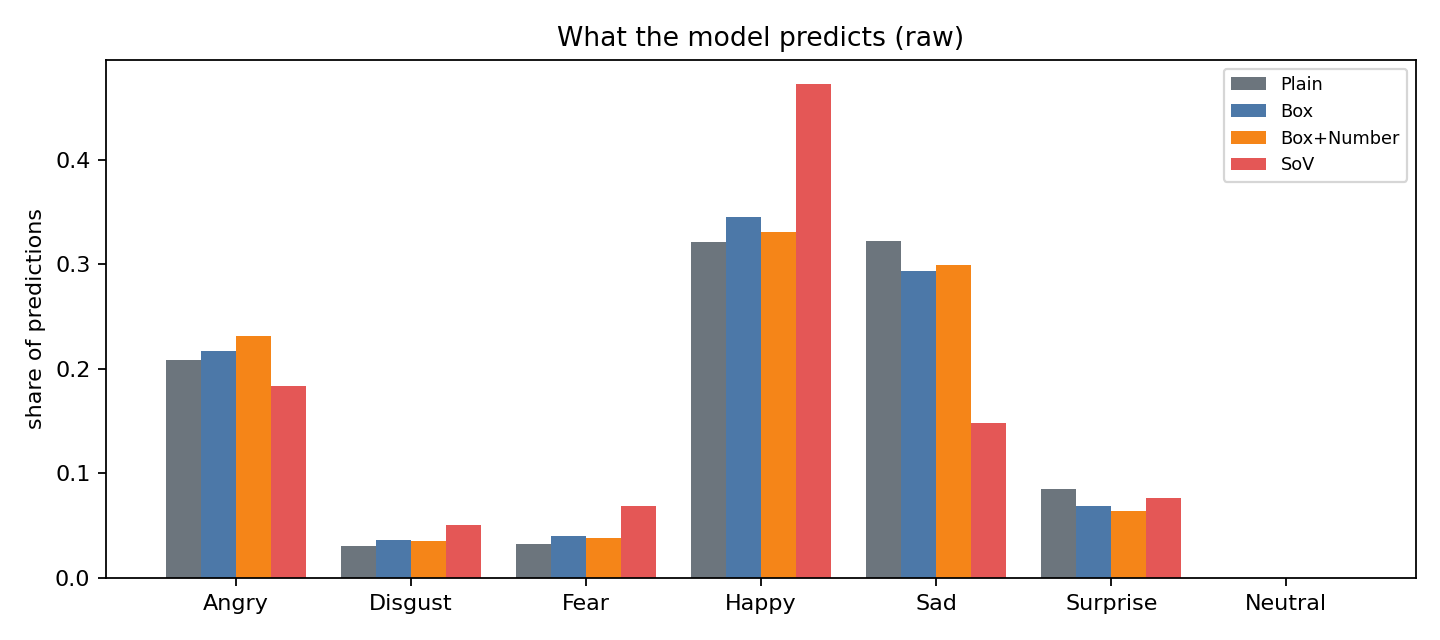
\includegraphics[width=\columnwidth]{core_llava_prediction_share.png}
\caption{Predicted-label shares for LLaVA across core visual conditions.}
\label{fig:sharellava}
\end{figure}
\begin{figure}[!t]
\centering
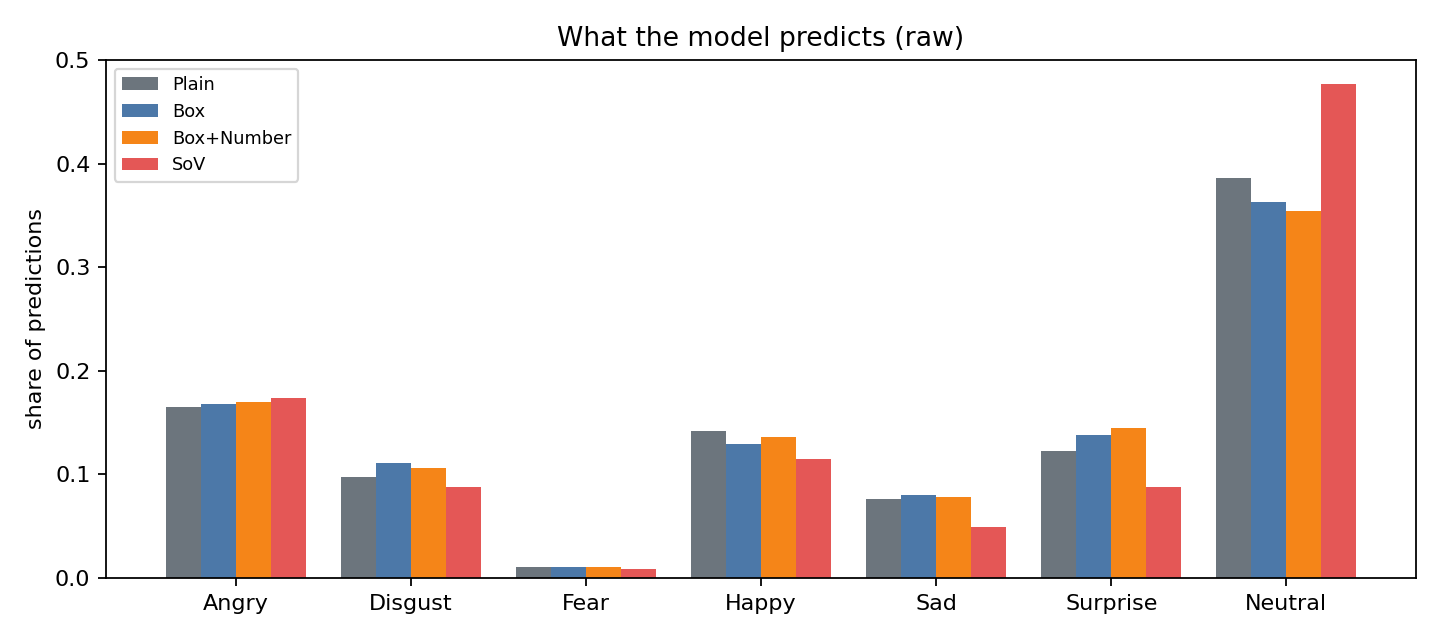
\includegraphics[width=\columnwidth]{core_qwen_prediction_share.png}
\caption{Predicted-label shares for Qwen across core visual conditions.}
\label{fig:shareqwen}
\end{figure}

\subsection{Per-emotion behaviour}
Per-emotion recall indicates that the aggregate changes are not uniform across classes. LLaVA has zero Neutral recall across the reported core conditions and shows changes concentrated particularly in Sad and Surprise. Qwen has substantially higher Neutral recall, while its SoV condition reduces recall for multiple classes, including Happy, Disgust, Sad, and Surprise. Selected per-class recall plots are provided in Fig.~\ref{fig:recallllava} and Fig.~\ref{fig:recallqwen}.

Table~\ref{tab:classcontrib} decomposes the paired SoV--Plain balanced-accuracy change by true emotion class. Each contribution is the class-specific recall change weighted by the class's equal contribution to balanced accuracy. The class contributions sum to the overall balanced-accuracy change.

\begin{table*}[!t]
\caption{Per-class contributions to the SoV--Plain balanced-accuracy change on the single-face core set, in percentage points.}
\label{tab:classcontrib}
\centering
\footnotesize
\begin{tabular}{lrrrr}
\toprule
Emotion & LLaVA recall change & LLaVA BA contribution & Qwen recall change & Qwen BA contribution \\
\midrule
Angry & $-6.7$ & $-0.95$ & $-1.3$ & $-0.19$ \\
Disgust & $+1.8$ & $+0.25$ & $-8.4$ & $-1.21$ \\
Fear & $+9.8$ & $+1.39$ & $-2.4$ & $-0.35$ \\
Happy & $-1.3$ & $-0.19$ & $-17.3$ & $-2.48$ \\
Sad & $-25.8$ & $-3.68$ & $-13.8$ & $-1.97$ \\
Surprise & $-15.6$ & $-2.22$ & $-16.9$ & $-2.41$ \\
Neutral & $0.0$ & $0.00$ & $+3.6$ & $+0.51$ \\
\midrule
Total & -- & $-5.40$ & -- & $-8.09$ \\
\bottomrule
\end{tabular}
\end{table*}


\begin{figure}[!t]
\centering
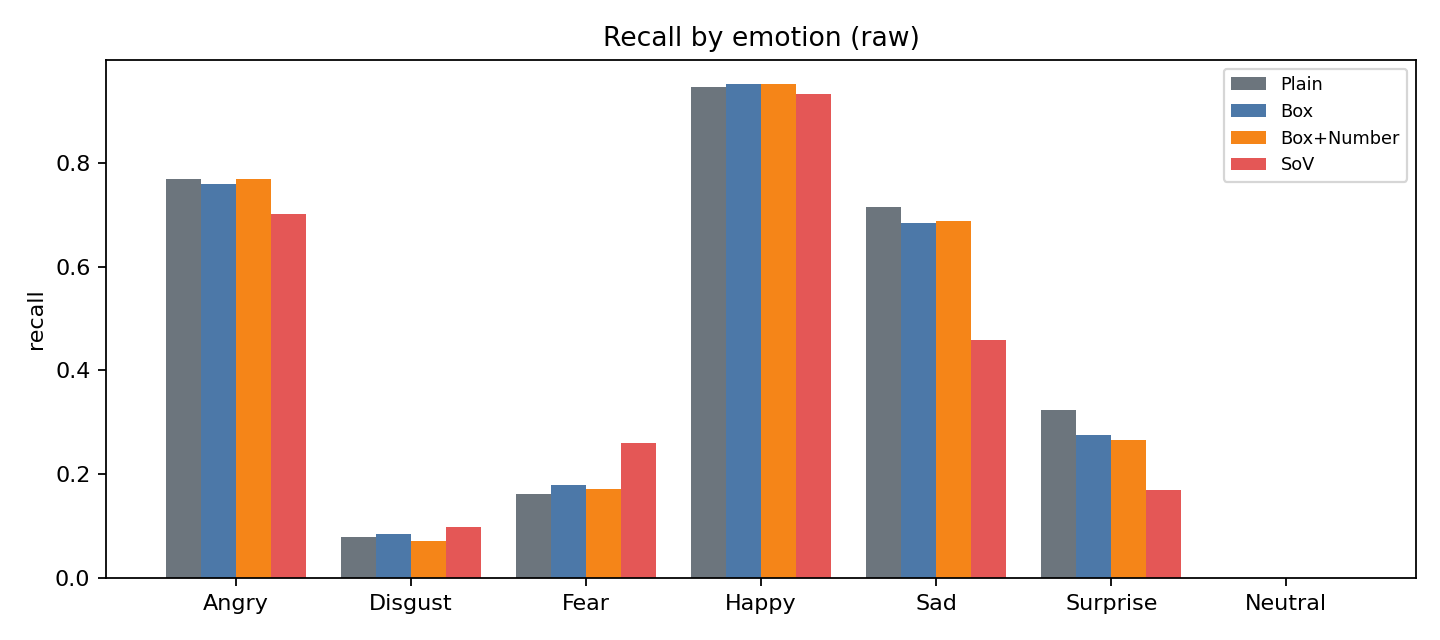
\includegraphics[width=\columnwidth]{core_llava_recall.png}
\caption{Per-emotion recall for LLaVA in the core set.}
\label{fig:recallllava}
\end{figure}
\begin{figure}[!t]
\centering
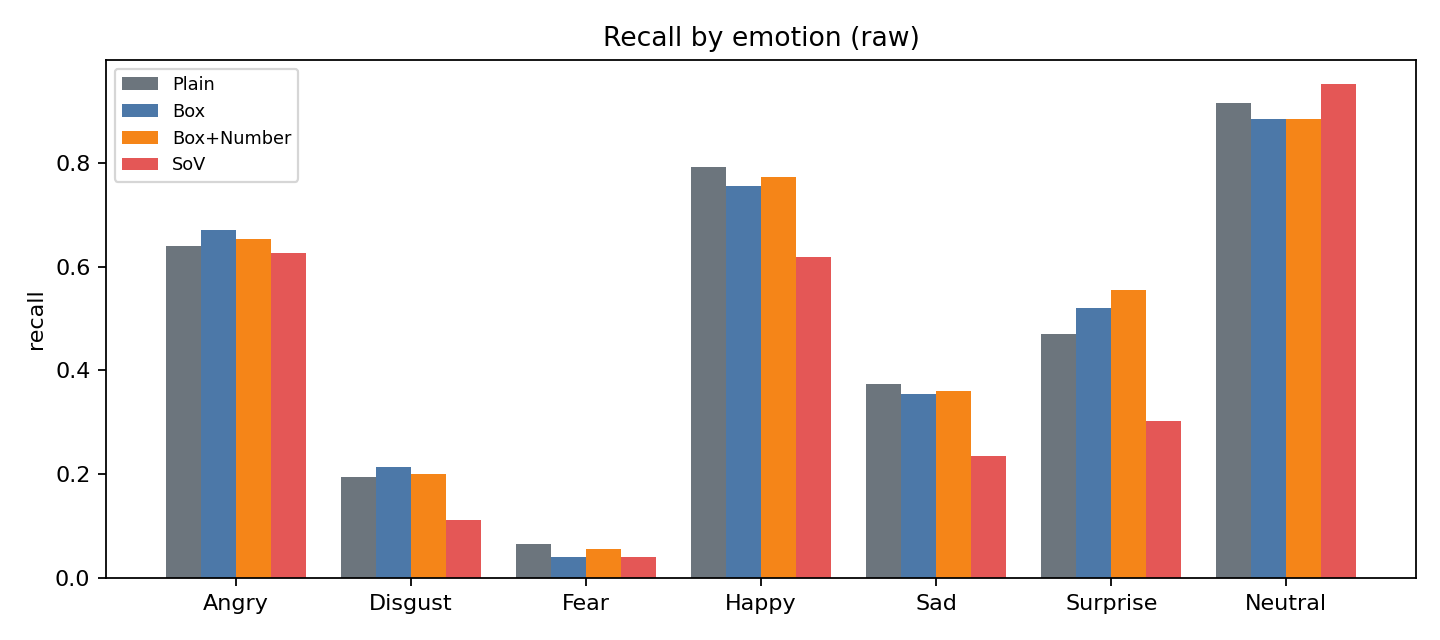
\includegraphics[width=\columnwidth]{core_qwen_recall.png}
\caption{Per-emotion recall for Qwen in the core set.}
\label{fig:recallqwen}
\end{figure}

\subsection{Demographic-group analysis}
The demographic analysis evaluates whether the SoV--Plain effect differs across FairFace-estimated groups. For the six-class group analysis, LLaVA's SoV--Plain differences are $-8.2$ pp for Caucasian-like faces (95\% CI: [$-11.2,-5.4$]), $-9.3$ pp for Asian faces ([$-12.7,-6.1$]), and $-6.2$ pp for Black faces ([$-9.6,-2.9$]). Qwen's corresponding differences are $-9.1$ pp ([$-13.2,-5.1$]), $-13.6$ pp ([$-17.3,-9.8$]), and $-4.4$ pp ([$-7.9,-0.9$]).

The between-group contrasts do not detect a race-group or gender difference in the SoV effect. For LLaVA, Asian versus Caucasian-like is $-1.1$ pp ([$-5.3,+2.8$]), Black versus Caucasian-like is $+2.0$ pp ([$-2.5,+6.3$]), and Female versus Male is $-1.2$ pp ([$-4.9,+2.7$]). For Qwen, the corresponding contrasts are $-4.4$ pp ([$-9.9,+1.0$]), $+4.7$ pp ([$-0.5,+10.0$]), and $+3.1$ pp ([$-1.6,+8.1$]). These intervals include zero, but they are not equivalence tests. In particular, Qwen's intervals permit group differences of several percentage points and in some cases approach ten points.

Age-band results are exploratory. One Qwen contrast, age 40--59 versus 20--29, is $+7.0$ pp ([$+0.2,+14.0$]); this is one borderline interval among multiple subgroup comparisons and should not be treated as a confirmed age effect. Face-size and crop-type patterns also differ between models and are treated as exploratory.

\begin{figure}[!t]
\centering
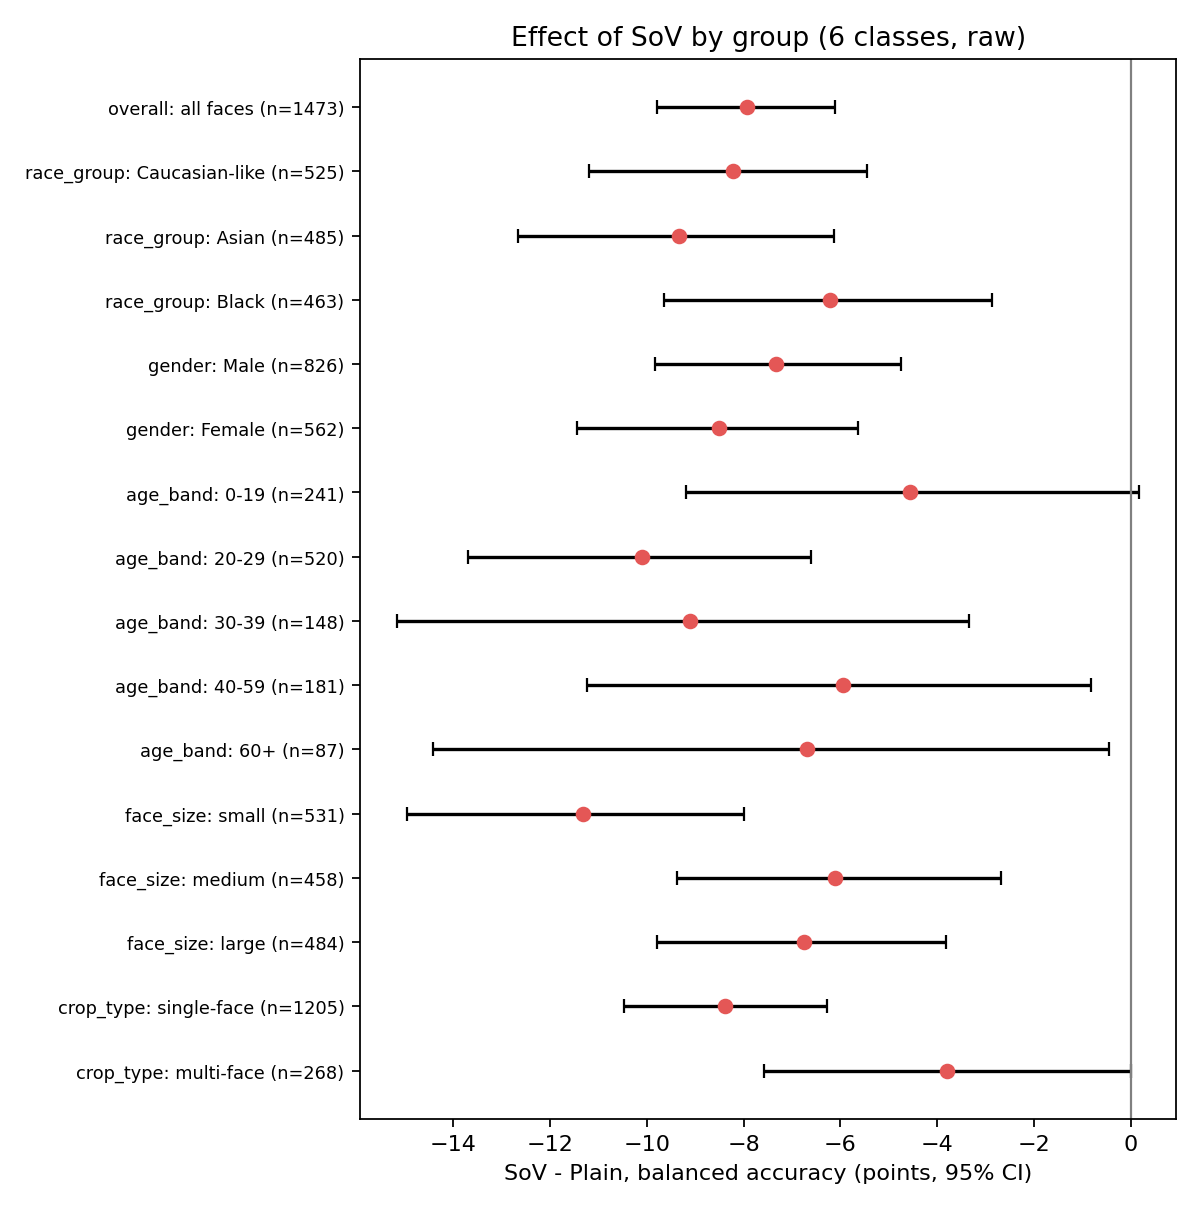
\includegraphics[width=\columnwidth]{core_llava_group_forest.png}
\caption{LLaVA SoV--Plain effects across estimated demographic and image subgroups.}
\label{fig:forestllava}
\end{figure}
\begin{figure}[!t]
\centering
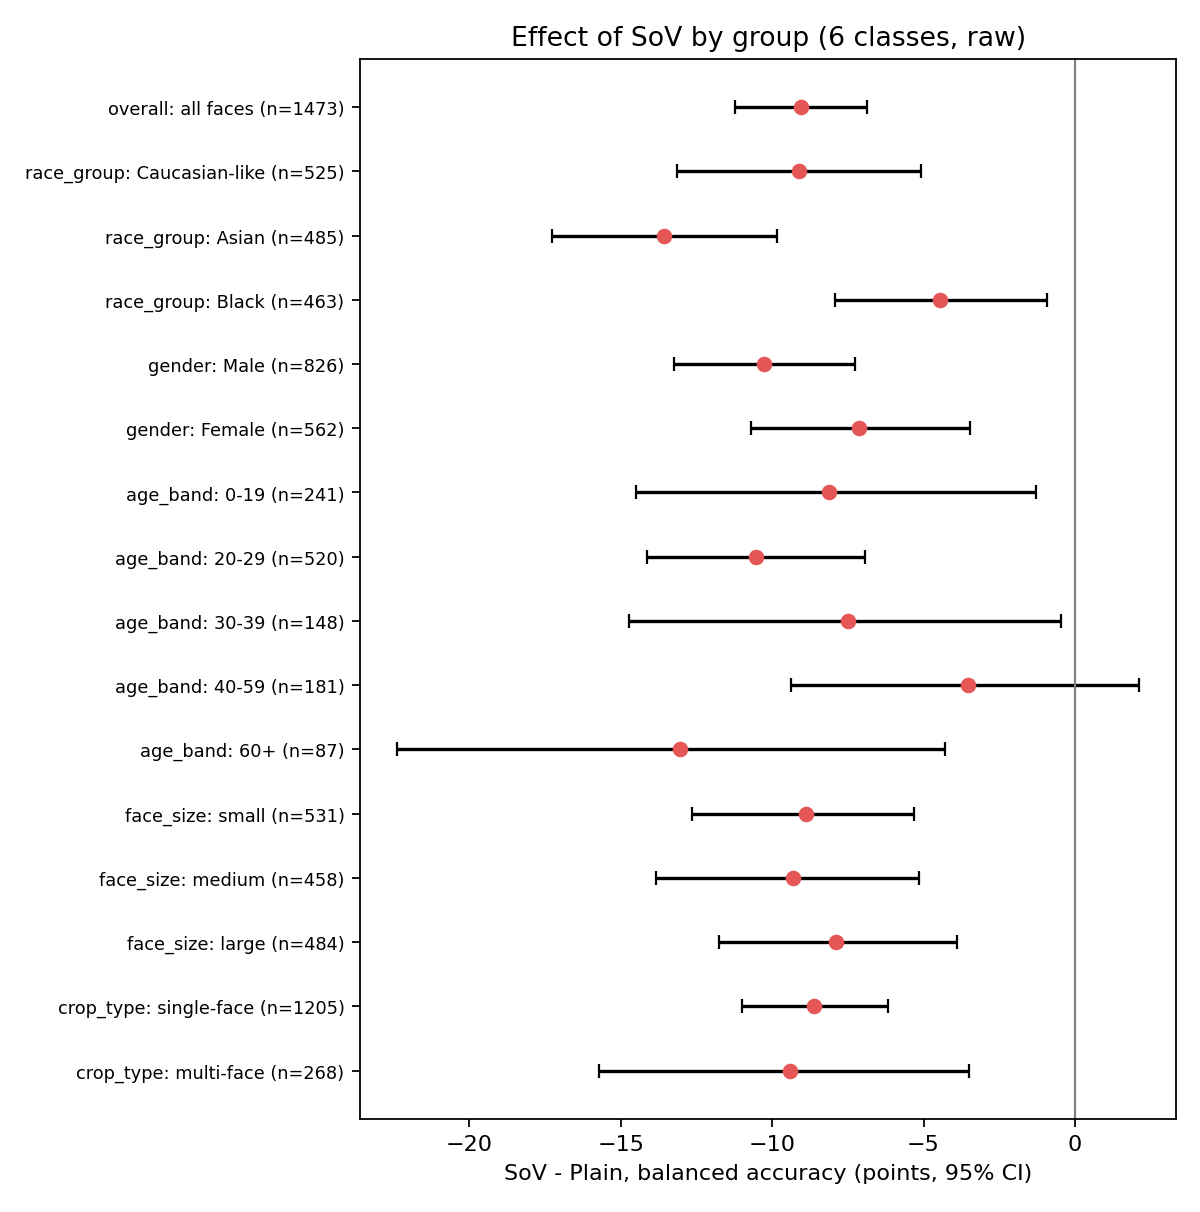
\includegraphics[width=\columnwidth]{core_qwen_group_forest.png}
\caption{Qwen SoV--Plain effects across estimated demographic and image subgroups.}
\label{fig:forestqwen}
\end{figure}

\subsection{Multi-face evaluation}
The multi-face set contains 2,816 scored target faces from 1,250 images. The pooled set is strongly imbalanced: approximately 64\% of the targets are Happy. We therefore report both all-face accuracy and the 301-face other-emotion subset (Angry, Disgust, Fear, Sad, and Surprise).

In the as-designed comparison, SoV minus Plain is $-1.2$ pp (95\% CI: [$-2.2,-0.3$]) for LLaVA and $-14.9$ pp ([$-17.0,-12.7$]) for Qwen. Box+Number minus Plain is $+0.6$ pp ([$-0.0,+1.2$]) for LLaVA and $+5.0$ pp ([$+3.3,+6.7$]) for Qwen. These as-designed contrasts change the visual condition and can also change the target-reference prompt. They describe the full arms and should not be interpreted as overlay-only effects.

The matched-prompt comparison isolates overlay changes more directly. With the numbered prompt held fixed, adding landmarks to Box+Number (SoV minus Box+Number) is $-1.8$ pp ([$-2.6,-1.1$]) for LLaVA and $-19.9$ pp ([$-21.9,-17.8$]) for Qwen across all faces. On the other-emotion subset, the corresponding differences are $-12.3$ pp ([$-16.9,-7.9$]) and $-14.3$ pp ([$-20.0,-8.7$]). These are matched-prompt contrasts and support an overlay-specific interpretation within the evaluated conditions.

For the other-emotion subset, the as-designed SoV--Plain difference is $-16.9$ pp ([$-23.3,-11.1$]) for LLaVA and $-13.3$ pp ([$-19.4,-7.5$]) for Qwen. These results indicate substantial difficulty on less frequent non-Happy classes, but the comparison remains as-designed and must not be used to attribute the full difference to the overlay alone.

Qwen's pooled multi-face behaviour is strongly influenced by Happy/Neutral confusions. Its Happy recall decreases from approximately 0.67 under Plain to 0.44 under SoV, while the share of Happy faces predicted as Neutral increases from about 32\% to 55\%. This helps explain why pooled accuracy changes sharply. It does not demonstrate that the model has failed to localize the correct face. LLaVA, by contrast, maintains Happy recall near 0.97--0.99 and never predicts Neutral in the reported multi-face arms.

\begin{figure}[!t]
\centering
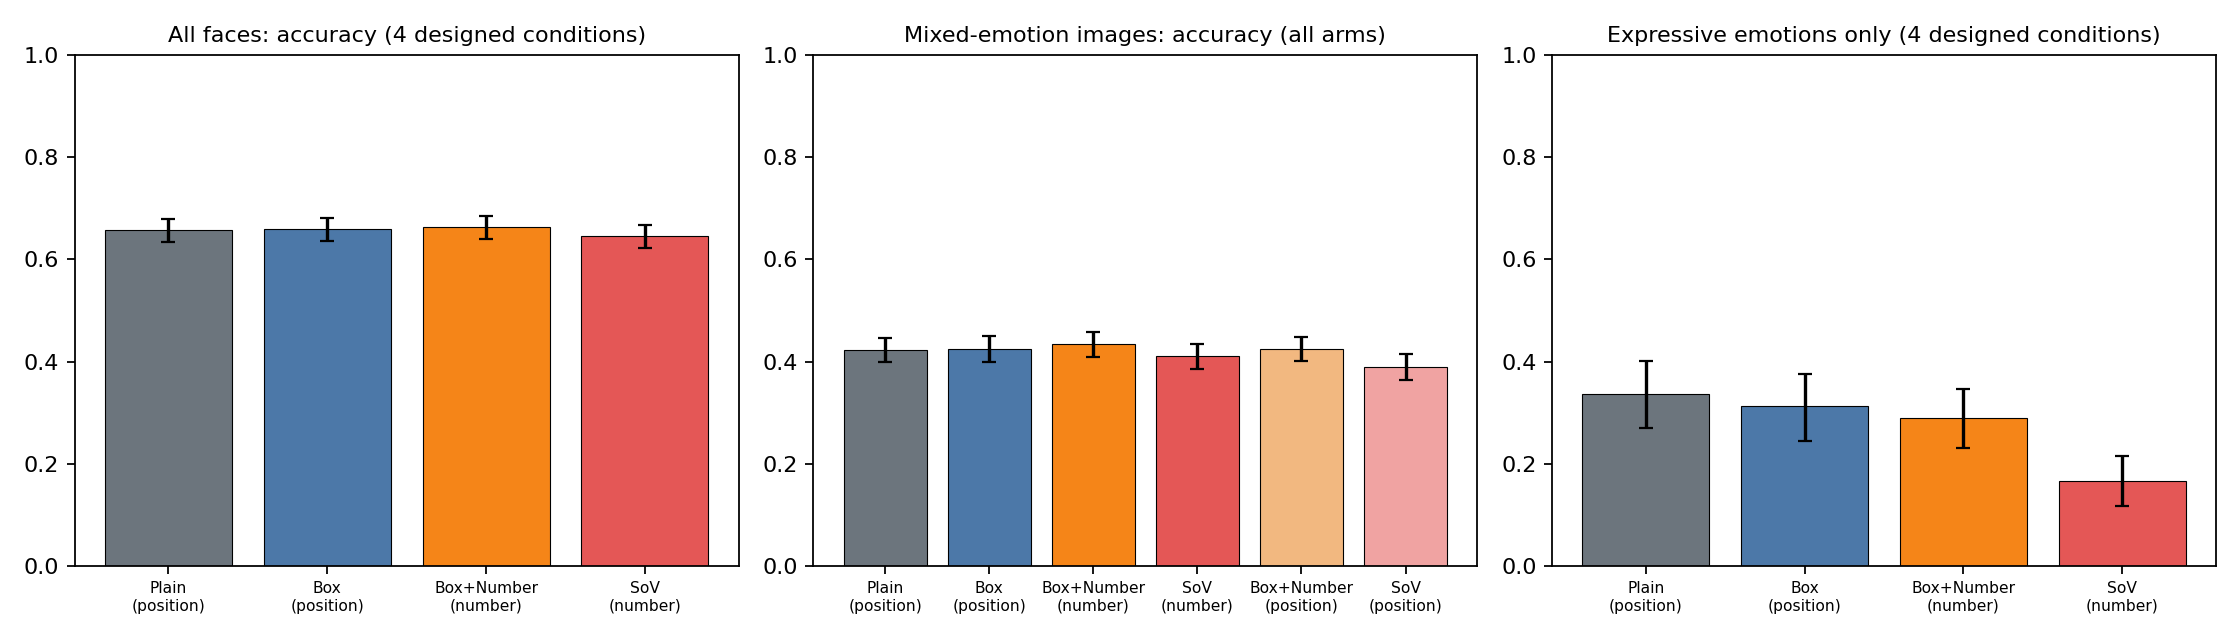
\includegraphics[width=\columnwidth]{multiface_llava_arms.png}
\caption{LLaVA multi-face accuracy by experimental arm.}
\label{fig:multillava}
\end{figure}
\begin{figure}[!t]
\centering
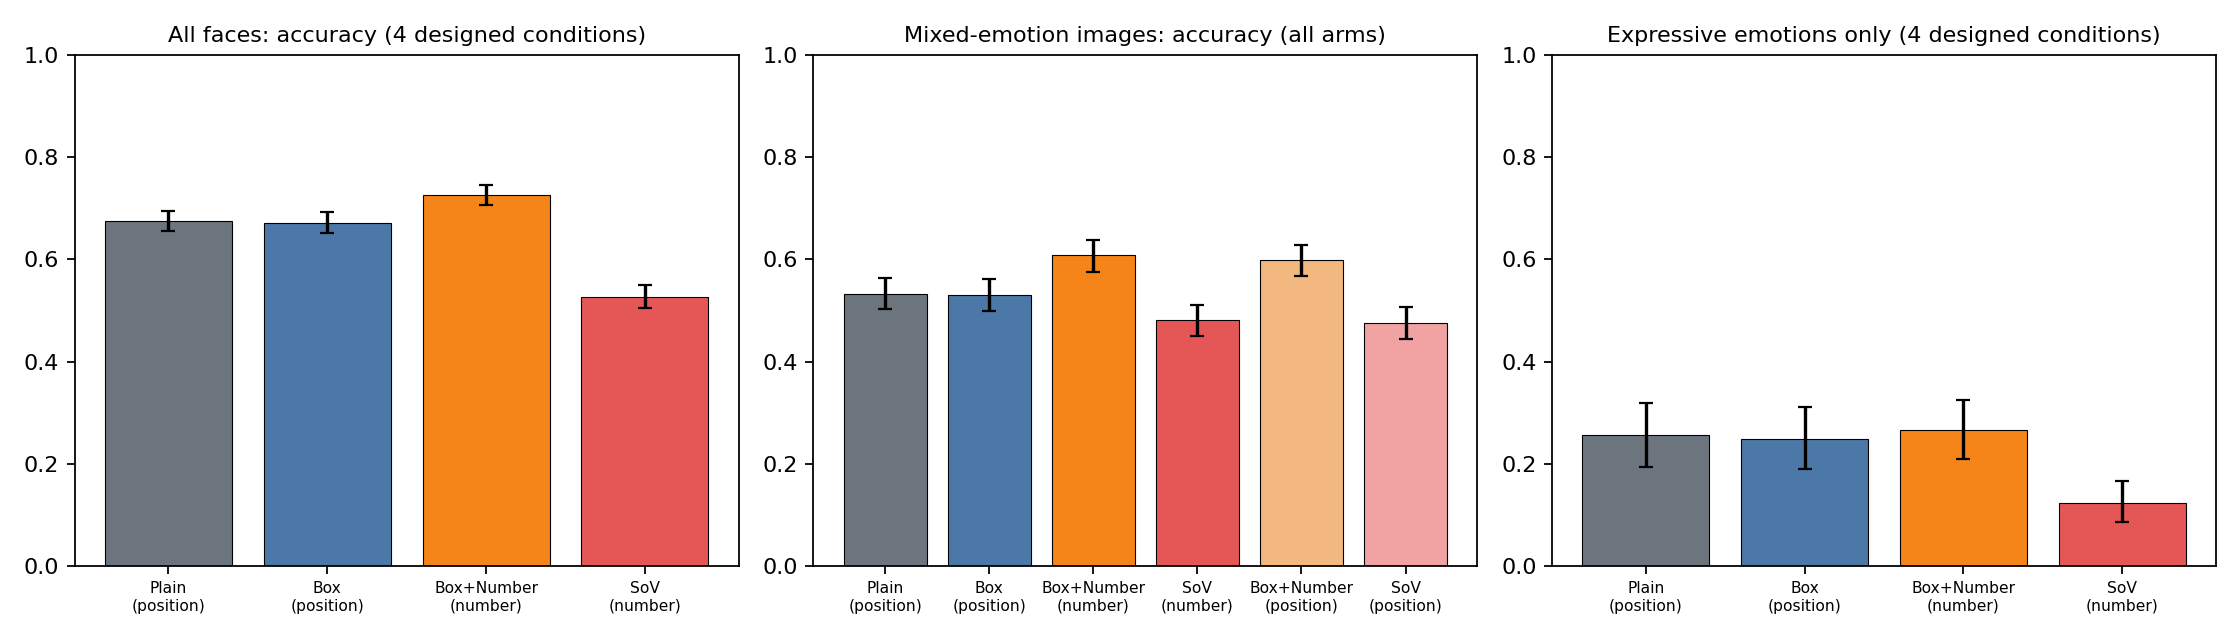
\includegraphics[width=\columnwidth]{multiface_qwen_arms.png}
\caption{Qwen multi-face accuracy by experimental arm.}
\label{fig:multiqwen}
\end{figure}

\subsection{Direct cross-model contrasts}
Direct LLaVA--Qwen contrasts were selected after both result sets were inspected and are therefore post hoc. In the core set, the Qwen-minus-LLaVA difference in the SoV--Plain effect is $-2.7$ pp (95\% CI: [$-5.3,-0.1$]), a borderline result. The corresponding multi-face as-designed difference is $-13.7$ pp ([$-15.8,-11.5$]). This does not justify ranking the models: their Neutral behaviour, label distributions, visual processing, and development-set procedures differ. Cross-model comparisons are included to describe differences in observed response to the conditions, not to claim general model superiority.

\section{Ablation and Additional Probes}
\subsection{Half-size landmark dots}
The half-dot SoV condition improves over full-dot SoV by $+2.6$ pp for LLaVA (95\% CI: [$+1.1,+4.0$]) and $+3.4$ pp for Qwen ([$+1.8,+4.8$]). However, half-dot SoV remains below Plain by $-2.8$ pp for LLaVA ([$-4.4,-1.2$]) and $-4.7$ pp for Qwen ([$-6.4,-3.0$]). The recovery is a little under half of the raw SoV--Plain reduction in both models. The result shows sensitivity to dot size, but it does not identify why the larger dots reduce performance.

\subsection{Numbered versus centre-based prompts}
On the 268 core faces whose context crop contains other faces, the numbered prompt does not produce a clear improvement for LLaVA: Box+Number numbered minus centre is $-0.7$ pp ([$-3.0,+1.3$]) and SoV numbered minus centre is $-0.7$ pp ([$-3.2,+1.8$]). For Qwen, the Box+Number difference is $+2.6$ pp ([$+0.0,+5.3$]), while the SoV difference is $+0.7$ pp ([$-2.4,+4.0$]). The sample is limited, and the estimates should be interpreted cautiously.

\subsection{Shuffled-tag reading probe}
The shuffled-tag probe reports exact-match rates of 0.63 for LLaVA under both Box+Number and SoV, and 0.782 and 0.755 for Qwen, respectively. Approximate chance is 0.23. LLaVA's rightmost-face exact match is lower than its leftmost-face match (0.45 versus 0.817 in Box+Number); Qwen's rates are 0.756 and 0.810, respectively. These results suggest that the models can read the numeric markers above chance on the probe, with different error patterns. They do not prove that tag reading caused any accuracy changes in the multi-face classification experiment. The probe is interpreted as a diagnostic of numeric-tag reading, not as a causal test of classification performance.

\section{Discussion}
The main finding is not that visual prompts universally fail, but that the tested SoV-style condition did not improve balanced accuracy in this particular pipeline. Raw SoV--Plain balanced accuracy was lower for both evaluated models. The Box and Box+Number conditions were close to Plain, suggesting that the large performance change appears at the cumulative step that adds landmark dots to the numbered-box condition. The half-dot ablation recovers part, but not all, of the difference.

The calibration results require model-specific interpretation. LLaVA's self-calibrated SoV--Plain interval includes zero, while Qwen's remains negative. It would therefore be inaccurate to state that the reduction persists equally after answer-bias correction in both models. Conversely, it would also be inaccurate to describe the entire raw reduction as answer bias: that interpretation is not supported for Qwen by the current self-calibrated analysis.

The multi-face experiment reinforces the need to separate prompt and overlay manipulations. An as-designed contrast can reflect both a changed image and a changed reference instruction. Matched-prompt contrasts are more informative about the overlay itself. In particular, the matched-prompt SoV--Box+Number contrast compares the addition of landmark dots while retaining the numbered prompt. These distinctions should be retained in all tables, captions, and discussion.

The demographic analysis does not detect a race-group or gender difference in the SoV effect in the core set. This is not evidence that the model is unbiased or that group effects are equivalent. The FairFace labels are predictions, the groups are operationally defined, and the confidence intervals—especially for Qwen—allow non-trivial differences. Age-related patterns are exploratory and should not be elevated to the main conclusion.

Several explanations for the landmark effect are plausible but untested. Dots may overlap expression-relevant regions, their apparent size may be large relative to a 336-pixel crop, or the implementation may differ from the original SoV overlay in ways that affect visual interpretation. The half-dot ablation indicates that marker size matters, but does not distinguish these mechanisms. These possibilities should be framed as hypotheses for future controlled experiments.

\section{Limitations}
\subsection{Dataset and annotation limitations}
ExpW is an in-the-wild dataset with noisy expression annotations. There is no human-performance ceiling in the current evaluation, so the attainable score under the annotation scheme is unknown. The dataset is also web-sourced and may not represent the range of image conditions or populations encountered in other settings. RAF-DB was not included because access was not obtained.

\subsection{Demographic-label limitations}
FairFace estimates race, gender, and age from facial images. These estimates are not ground truth and can contain systematic error. Agreement across two crop paddings measures stability, not correctness. The final analysis uses operational race groups and excludes or does not separately represent some FairFace categories. Group-by-emotion cells are small for several labels, particularly outside Happy. The results cannot support claims about true ethnicity, culture, or nationality.

\subsection{Model and implementation limitations}
Only two 7B-class open VLMs were evaluated, and both used 4-bit quantization. No full-precision comparison was run. The SoV overlay is the project's own approximation and should not be presented as an exact reproduction of the official implementation. Context crops were used instead of full images. Although the crops have a nominal size of 336 by 336, the two model families process visual inputs differently. Qwen was not dev-gated and has no dev-calibrated result. LLaVA and Qwen also differ substantially in Neutral-label behaviour.

\subsection{Experimental-design and statistical limitations}
The overlay conditions are cumulative rather than factorial, so independent component effects and interactions cannot all be identified. The half-dot analysis was announced after initial results. Many subgroup and cross-model comparisons were conducted; borderline intervals are exploratory. No equivalence margin was specified. The multi-face sample is dominated by Happy and Neutral labels, and only a small subset contains other emotion classes.

\section{Conclusion and Future Work}
Under our experimental setup, SoV did not improve balanced accuracy. The raw performance reduction was observed in both models, although its persistence after answer-bias correction differed between models. Box and Box+Number were close to Plain, while adding landmark dots to Box+Number reduced balanced accuracy. Half-size dots recovered a little under half of the raw reduction but did not eliminate it. The core analysis did not detect a race-group or gender difference in the SoV effect; the intervals do not establish equivalence. Multi-face findings depend on whether the prompt is held fixed, and pooled accuracy is strongly affected by class imbalance and model-specific Neutral behaviour.

Future work should test the official SoV overlay specification, use a factorial design to isolate boxes, numbers, and landmarks, and evaluate full-image and higher-resolution inputs. Additional models and full-precision comparisons would help assess whether the observed patterns generalize. Better-balanced multi-face data and human-verified or self-reported demographic annotations would strengthen subgroup analysis. Any future fairness claims should specify an equivalence margin in advance and use sufficiently large subgroup samples.

\section{Code Availability}
The project implementation and associated materials are available in the project repository:
\url{https://github.com/varunbabuvb/ml_project}. Dataset access remains subject to the original ExpW distribution terms. The reported results were generated using the model configurations and evaluation subsets described in this paper.


\appendices

\section{Exact Prompts Used}
\label{app:prompts}
Prompt variant A (without a Neutral hint) was used for the core and multi-face evaluations. Each prompt requests exactly one of the seven expression labels. Predictions are obtained by scoring the candidate-label token sequences rather than by accepting unconstrained free-text generation. The scoring implementation sums the capitalised, lower-case, and space-prefixed token variants for each label.

\textbf{Single-face centre prompt}, used for the four principal visual conditions and the half-dot condition:
\begin{quote}\small
What is the emotion of the person in the center of the image? Choose exactly one of: Angry, Disgust, Fear, Happy, Sad, Surprise, Neutral. Answer with the emotion word only.
\end{quote}

\textbf{Numbered prompt}, used for Box+Number and SoV in the multi-face experiment and for the numbered-query jobs on core crops containing additional faces:
\begin{quote}\small
What is the emotion of the person labeled ``$k$''? Choose exactly one of: Angry, Disgust, Fear, Happy, Sad, Surprise, Neutral. Answer with the emotion word only.
\end{quote}
Here, $k$ is replaced by the numeric identifier printed on the target face.

\textbf{Positional prompt}, used for Plain and Box in the multi-face experiment and for the matched-prompt positional-query arms:
\begin{quote}\small
What is the emotion of the $N$th face from the left? Choose exactly one of: Angry, Disgust, Fear, Happy, Sad, Surprise, Neutral. Answer with the emotion word only.
\end{quote}
Here, $N$ is replaced by the target face's ordinal position from the left (for example, ``first'', ``second'', or ``third'').

A second wording (variant B), which adds the instruction ``Use `Neutral' when the face shows no clear emotion'', was evaluated on the development set only. Variant A was selected using the pre-specified mean macro-F1 rule over Plain and SoV (Appendix~\ref{app:dev}). Variant B was not used for the core or multi-face results.

\section{Additional Demographic-Group Results and Sample Sizes}
\label{app:groups}
Values are percentage-point differences in balanced accuracy (SoV minus Plain), with 95\% image-cluster bootstrap intervals. The single-face subgroup tables use raw scores and the six-class set that excludes Fear because of small group-by-emotion cells. Group labels are FairFace estimates (Appendix~\ref{app:fairface}). Race and gender are the pre-specified subgroup analyses; age, face-size, and crop-type rows are exploratory. An asterisk marks an interval that excludes zero. Given the number of comparisons, isolated borderline intervals are not interpreted as confirmatory findings.

\subsection{Single-face core set: SoV minus Plain by subgroup}
\begin{table*}[!t]
\caption{Core set: SoV minus Plain (pp) by subgroup. $n$ is the number of faces.}
\label{tab:app_groups_core}
\centering
\scriptsize
\setlength{\tabcolsep}{3pt}
\begin{tabular}{lrcc}
\toprule
Subgroup & $n$ & LLaVA-1.5-7B & Qwen2.5-VL-7B \\
\midrule
All faces & 1,473 & $-7.9$ [$-9.8$, $-6.1$] & $-9.0$ [$-11.2$, $-6.9$] \\
Caucasian-like & 525 & $-8.2$ [$-11.2$, $-5.4$] & $-9.1$ [$-13.2$, $-5.1$] \\
Asian & 485 & $-9.3$ [$-12.7$, $-6.1$] & $-13.6$ [$-17.3$, $-9.8$] \\
Black & 463 & $-6.2$ [$-9.6$, $-2.9$] & $-4.4$ [$-7.9$, $-0.9$] \\
Male & 826 & $-7.3$ [$-9.8$, $-4.8$] & $-10.3$ [$-13.2$, $-7.3$] \\
Female & 562 & $-8.5$ [$-11.4$, $-5.6$] & $-7.1$ [$-10.7$, $-3.5$] \\
\midrule
Age 0--19 & 241 & $-4.6$ [$-9.2$, $+0.2$] & $-8.1$ [$-14.5$, $-1.3$] \\
Age 20--29 & 520 & $-10.1$ [$-13.7$, $-6.6$] & $-10.5$ [$-14.1$, $-6.9$] \\
Age 30--39 & 148 & $-9.1$ [$-15.2$, $-3.3$] & $-7.5$ [$-14.7$, $-0.5$] \\
Age 40--59 & 181 & $-6.0$ [$-11.2$, $-0.8$] & $-3.5$ [$-9.4$, $+2.1$] \\
Age 60+ (small) & 87 & $-6.7$ [$-14.4$, $-0.5$] & $-13.1$ [$-22.4$, $-4.3$] \\
\midrule
Face size: small & 531 & $-11.3$ [$-15.0$, $-8.0$] & $-8.9$ [$-12.7$, $-5.3$] \\
Face size: medium & 458 & $-6.1$ [$-9.4$, $-2.7$] & $-9.3$ [$-13.8$, $-5.2$] \\
Face size: large & 484 & $-6.8$ [$-9.8$, $-3.8$] & $-7.9$ [$-11.8$, $-3.9$] \\
\midrule
Crop: single-face & 1,205 & $-8.4$ [$-10.5$, $-6.3$] & $-8.6$ [$-11.0$, $-6.2$] \\
Crop: multi-face & 268 & $-3.8$ [$-7.6$, $0.0$] & $-9.4$ [$-15.7$, $-3.5$] \\
\bottomrule
\end{tabular}
\end{table*}

\subsection{Single-face core set: between-group differences in the SoV effect}
Each row is the SoV--Plain effect in the stated group minus the effect in the reference group.
\begin{table*}[!t]
\caption{Core set: between-group differences in the SoV--Plain effect (pp).}
\label{tab:app_groups_diff}
\centering
\scriptsize
\setlength{\tabcolsep}{3pt}
\begin{tabular}{lcc}
\toprule
Contrast & LLaVA-1.5-7B & Qwen2.5-VL-7B \\
\midrule
Asian vs Caucasian-like & $-1.1$ [$-5.3$, $+2.8$] & $-4.4$ [$-9.9$, $+1.0$] \\
Black vs Caucasian-like & $+2.0$ [$-2.5$, $+6.3$] & $+4.7$ [$-0.5$, $+10.0$] \\
Female vs Male & $-1.2$ [$-4.9$, $+2.7$] & $+3.1$ [$-1.6$, $+8.1$] \\
\midrule
Age 0--19 vs 20--29 & $+5.5$ [$0.0$, $+11.3$]$^{*}$ & $+2.4$ [$-4.7$, $+10.1$] \\
Age 30--39 vs 20--29 & $+1.0$ [$-5.7$, $+7.7$] & $+3.0$ [$-5.4$, $+11.3$] \\
Age 40--59 vs 20--29 & $+4.2$ [$-2.2$, $+10.4$] & $+7.0$ [$+0.2$, $+14.0$]$^{*}$ \\
Age 60+ vs 20--29 & $+3.4$ [$-4.7$, $+10.6$] & $-2.5$ [$-12.8$, $+7.0$] \\
\midrule
Face size: medium vs small & $+5.2$ [$+0.5$, $+10.3$]$^{*}$ & $-0.4$ [$-6.3$, $+5.4$] \\
Face size: large vs small & $+4.6$ [$+0.2$, $+9.1$]$^{*}$ & $+1.0$ [$-4.1$, $+6.5$] \\
Crop: multi vs single-face & $+4.6$ [$+0.2$, $+8.7$]$^{*}$ & $-0.8$ [$-7.8$, $+5.6$] \\
\bottomrule
\end{tabular}
\end{table*}

\subsection{Multi-face set: between-group differences in the as-designed SoV--Plain effect}
The multi-face rows use the as-designed contrast (SoV with numbered prompt minus Plain with positional prompt) on all scored faces. Because this contrast changes the overlay and prompt together, it is used only to compare subgroup effects and not to attribute differences to the overlay mechanism.
\begin{table*}[!t]
\caption{Multi-face set: between-group differences in the as-designed SoV--Plain effect (pp). All rows are exploratory.}
\label{tab:app_groups_multi}
\centering
\scriptsize
\setlength{\tabcolsep}{3pt}
\begin{tabular}{lcc}
\toprule
Contrast & LLaVA-1.5-7B & Qwen2.5-VL-7B \\
\midrule
Asian vs Caucasian-like & $+1.1$ [$-1.0$, $+3.0$] & $+0.9$ [$-4.2$, $+6.0$] \\
Black vs Caucasian-like & $+1.2$ [$-1.3$, $+3.8$] & $+2.4$ [$-3.6$, $+9.0$] \\
Male vs Female & $0.0$ [$-1.5$, $+1.5$] & $+0.8$ [$-3.0$, $+4.7$] \\
\midrule
Age 0--19 vs 20--29 & $-0.6$ [$-3.0$, $+1.8$] & $+0.6$ [$-5.5$, $+6.6$] \\
Age 30--39 vs 20--29 & $+0.4$ [$-2.8$, $+3.3$] & $-0.6$ [$-7.3$, $+5.6$] \\
Age 40--59 vs 20--29 & $+0.3$ [$-2.4$, $+3.1$] & $-6.8$ [$-13.5$, $-0.6$]$^{*}$ \\
Age 60+ vs 20--29 & $-0.9$ [$-6.1$, $+4.3$] & $-8.1$ [$-16.8$, $+0.6$] \\
\midrule
Face size: medium vs small & $+0.7$ [$-1.9$, $+3.3$] & $+14.0$ [$+8.4$, $+19.2$]$^{*}$ \\
Face size: large vs small & $+2.0$ [$-0.3$, $+4.6$] & $+25.7$ [$+20.7$, $+30.4$]$^{*}$ \\
Image: mixed vs not mixed & $0.0$ [$-2.2$, $+2.0$] & $+15.0$ [$+10.9$, $+19.1$]$^{*}$ \\
Detections $\neq$ targets vs equal & $-0.6$ [$-2.8$, $+1.3$] & $-2.3$ [$-6.7$, $+2.4$] \\
3+ targets vs 2 targets & $-1.5$ [$-4.3$, $+1.0$] & $-18.3$ [$-23.6$, $-13.0$]$^{*}$ \\
\bottomrule
\end{tabular}
\end{table*}

\subsection{Group sample sizes and small cells}
In the core set, each race-group by emotion cell contains 75 faces for the six non-Fear emotions. Fear contains 75, 35, and 13 faces for the Caucasian-like, Asian, and Black groups, respectively; the Black--Fear cell (13 faces) is below the 30-face threshold and is flagged. Fear is excluded from the group tables above.

In the multi-face set, cells below 30 faces outside Happy and Neutral include Asian--Angry (5), Asian--Disgust (13), Asian--Fear (0), Asian--Sad (20), Asian--Surprise (17), Black--Angry (0), Black--Disgust (11), Black--Fear (0), Black--Sad (4), Black--Surprise (7), and Caucasian-like--Fear (9). Group-specific claims about non-Happy expressions in the multi-face set are therefore not supported. In the core set, the median face-box size is approximately 114 pixels for faces estimated as Black and 135 pixels for the other two race groups, so face size and estimated group are partly confounded.

\section{Per-Emotion Recall Tables}
\label{app:recall}
Recall is the proportion of faces with a given true label that the model predicts correctly. P = Plain, B = Box, B+N = Box+Number, S = SoV, and H = half-dot SoV.

\subsection{Single-face core set}
\begin{table*}[!t]
\caption{Core-set per-emotion recall (seven classes, raw scores).}
\label{tab:app_recall_core}
\centering
\scriptsize
\setlength{\tabcolsep}{3pt}
\begin{tabular}{lccccc|ccccc}
\toprule
& \multicolumn{5}{c|}{LLaVA-1.5-7B} & \multicolumn{5}{c}{Qwen2.5-VL-7B} \\
Emotion & P & B & B+N & S & H & P & B & B+N & S & H \\
\midrule
Angry & 0.77 & 0.76 & 0.77 & 0.70 & 0.78 & 0.64 & 0.67 & 0.65 & 0.63 & 0.63 \\
Disgust & 0.08 & 0.08 & 0.07 & 0.10 & 0.07 & 0.20 & 0.21 & 0.20 & 0.11 & 0.14 \\
Fear & 0.16 & 0.18 & 0.17 & 0.26 & 0.23 & 0.07 & 0.04 & 0.06 & 0.04 & 0.04 \\
Happy & 0.95 & 0.95 & 0.95 & 0.93 & 0.96 & 0.79 & 0.76 & 0.77 & 0.62 & 0.68 \\
Sad & 0.72 & 0.68 & 0.69 & 0.46 & 0.57 & 0.37 & 0.36 & 0.36 & 0.24 & 0.30 \\
Surprise & 0.32 & 0.28 & 0.27 & 0.17 & 0.19 & 0.47 & 0.52 & 0.56 & 0.30 & 0.41 \\
Neutral & 0.00 & 0.00 & 0.00 & 0.00 & 0.00 & 0.92 & 0.88 & 0.88 & 0.95 & 0.92 \\
\bottomrule
\end{tabular}
\end{table*}

LLaVA's SoV loss is concentrated in Sad and Surprise. Qwen's loss is distributed across several classes, including Happy, while its Neutral recall remains between 0.88 and 0.95. LLaVA's Neutral recall is zero in every condition. Fear has only 123 core faces and Disgust recall is low for both models; changes in those rows should therefore be interpreted cautiously.

\subsection{Predicted-label distribution in the core set}
\begin{table*}[!t]
\caption{Share of core-set predictions by label (rounded; rows may sum to 0.99--1.01).}
\label{tab:app_shares}
\centering
\scriptsize
\setlength{\tabcolsep}{3pt}
\begin{tabular}{llccccccc}
\toprule
Model & Condition & Ang. & Dis. & Fear & Hap. & Sad & Sur. & Neu. \\
\midrule
LLaVA-1.5-7B & Plain & 0.21 & 0.03 & 0.03 & 0.32 & 0.32 & 0.09 & 0.00 \\
& Box & 0.22 & 0.04 & 0.04 & 0.34 & 0.29 & 0.07 & 0.00 \\
& Box+Number & 0.23 & 0.04 & 0.04 & 0.33 & 0.30 & 0.06 & 0.00 \\
& SoV & 0.18 & 0.05 & 0.07 & 0.47 & 0.15 & 0.08 & 0.00 \\
\midrule
Qwen2.5-VL-7B & Plain & 0.16 & 0.10 & 0.01 & 0.14 & 0.08 & 0.12 & 0.39 \\
& Box & 0.17 & 0.11 & 0.01 & 0.13 & 0.08 & 0.14 & 0.36 \\
& Box+Number & 0.17 & 0.11 & 0.01 & 0.14 & 0.08 & 0.15 & 0.35 \\
& SoV & 0.17 & 0.09 & 0.01 & 0.12 & 0.05 & 0.09 & 0.48 \\
\bottomrule
\end{tabular}
\end{table*}

\subsection{Multi-face set}
The recall table uses the 2,816 scored faces. Class sizes are Angry 37, Disgust 69, Fear 9, Happy 1,805, Sad 92, Surprise 94, and Neutral 710. Recall for Fear and Angry is based on few faces. Plain and Box use the positional prompt; Box+Number and SoV use the numbered prompt.
\begin{table*}[!t]
\caption{Multi-face per-emotion recall.}
\label{tab:app_recall_multi}
\centering
\scriptsize
\setlength{\tabcolsep}{3pt}
\begin{tabular}{llccccccc}
\toprule
Model & Arm & Ang. & Dis. & Fear & Hap. & Sad & Sur. & Neu. \\
\midrule
LLaVA-1.5-7B & Plain & 0.35 & 0.03 & 0.00 & 0.97 & 0.66 & 0.27 & 0.00 \\
& Box & 0.38 & 0.01 & 0.11 & 0.98 & 0.63 & 0.21 & 0.00 \\
& Box+Number & 0.46 & 0.01 & 0.00 & 0.99 & 0.53 & 0.21 & 0.00 \\
& SoV & 0.30 & 0.01 & 0.11 & 0.98 & 0.37 & 0.03 & 0.00 \\
\midrule
Qwen2.5-VL-7B & Plain & 0.30 & 0.06 & 0.33 & 0.67 & 0.16 & 0.47 & 0.87 \\
& Box & 0.32 & 0.06 & 0.22 & 0.67 & 0.14 & 0.47 & 0.85 \\
& Box+Number & 0.41 & 0.06 & 0.11 & 0.75 & 0.18 & 0.46 & 0.87 \\
& SoV & 0.22 & 0.07 & 0.11 & 0.44 & 0.09 & 0.16 & 0.93 \\
\bottomrule
\end{tabular}
\end{table*}

\begin{table*}[!t]
\caption{Predictions for Happy faces in the multi-face set (shares of the 1,805 Happy faces).}
\label{tab:app_happy}
\centering
\scriptsize
\setlength{\tabcolsep}{3pt}
\begin{tabular}{llccc}
\toprule
Model & Arm & Happy & Neutral & Other \\
\midrule
LLaVA-1.5-7B & Plain & 0.97 & 0.00 & 0.03 \\
& Box & 0.98 & 0.00 & 0.02 \\
& Box+Number & 0.99 & 0.00 & 0.01 \\
& SoV & 0.98 & 0.00 & 0.02 \\
\midrule
Qwen2.5-VL-7B & Plain & 0.67 & 0.32 & 0.01 \\
& Box & 0.67 & 0.31 & 0.02 \\
& Box+Number & 0.75 & 0.24 & 0.02 \\
& SoV & 0.44 & 0.55 & 0.01 \\
\bottomrule
\end{tabular}
\end{table*}

\section{Development-Set Selection and Calibration Details}
\label{app:dev}
\subsection{Development set}
The development set contains 280 faces (40 per emotion) from 279 images and is image-disjoint from the core set. It was used to check model behaviour, select between two prompt wordings, and fit an optional calibration vector. No selection was performed on the core set. The LLaVA development run contains 1,120 scored jobs (280 faces across four conditions).

\subsection{Development gate and prompt selection for LLaVA}
\begin{itemize}
\item \textbf{Gate:} Plain macro-F1 on the development set was 0.361, above the pre-set minimum of 0.25.
\item \textbf{Scoring check:} the scored label matched the model's generated answer on 99.3\% of development jobs, and 98.6\% of probability mass was assigned to the seven candidate expression labels.
\item \textbf{Prompt rule:} variant A was selected using the pre-specified mean macro-F1 over Plain and SoV: 0.323 for A and 0.310 for B.
\item \textbf{Neutral:} raw Neutral recall was zero in every condition; development-calibrated Neutral recall was approximately 0.35.
\end{itemize}
Qwen2.5-VL-7B-Instruct was not subjected to this gate and has no development run. There is therefore no development-calibrated Qwen result, and the two models did not follow identical model-selection procedures.

\subsection{Scoring variants}
\begin{itemize}
\item \textbf{Raw:} the highest-scoring candidate label, without correction.
\item \textbf{Self-calibrated:} for each condition, the seven candidate scores are adjusted by subtracting the log of that condition's mean predicted class distribution on the core set. This is label-free and applied condition-wise. It assumes that the mean prediction distribution is a useful estimate of answer preference; it is not a general correction for model bias.
\item \textbf{Development-calibrated (LLaVA only):} the same adjustment is estimated from the development set and applied to the corresponding core condition.
\end{itemize}
More explicitly, if $\ell_{ic}$ is the vector of seven candidate scores for image-face instance $i$ in condition $c$, then
\[
\tilde{\ell}_{ic}=\ell_{ic}-\log\left(\frac{1}{n_c}
\sum_{i=1}^{n_c}\operatorname{softmax}(\ell_{ic})\right),
\]
where the logarithm and subtraction are element-wise. For the development-calibrated variant, the average is computed over the development examples rather than the core examples.

\begin{table*}[!t]
\caption{Core-set balanced accuracy by scoring variant. P = Plain, B = Box, B+N = Box+Number, S = SoV.}
\label{tab:app_levels}
\centering
\scriptsize
\setlength{\tabcolsep}{3pt}
\begin{tabular}{lcccc|cccc}
\toprule
& \multicolumn{4}{c|}{LLaVA-1.5-7B} & \multicolumn{4}{c}{Qwen2.5-VL-7B} \\
Variant & P & B & B+N & S & P & B & B+N & S \\
\midrule
Raw, seven classes & .428 & .419 & .417 & .374 & .493 & .492 & .498 & .412 \\
Raw, no Neutral & .500 & .489 & .486 & .437 & .423 & .426 & .433 & .322 \\
Self-calibrated, seven classes & .468 & .483 & .482 & .446 & .514 & .514 & .509 & .448 \\
\bottomrule
\end{tabular}
\end{table*}

\begin{table*}[!t]
\caption{Core set: SoV minus Plain (pp) under each scoring variant.}
\label{tab:app_sov_variants}
\centering
\scriptsize
\setlength{\tabcolsep}{3pt}
\begin{tabular}{lcc}
\toprule
Variant & LLaVA-1.5-7B & Qwen2.5-VL-7B \\
\midrule
Raw, seven classes & $-5.4$ [$-7.3$, $-3.5$] & $-8.1$ [$-10.0$, $-6.2$] \\
Raw, no Neutral & $-6.3$ [$-8.5$, $-4.1$] & $-10.0$ [$-12.1$, $-7.9$] \\
Self-calibrated, seven classes & $-2.2$ [$-4.4$, $+0.1$] & $-6.5$ [$-8.8$, $-4.3$] \\
Self-calibrated, no Neutral & $-0.8$ [$-3.1$, $+1.7$] & $-8.1$ [$-10.4$, $-5.7$] \\
Development-calibrated, seven classes & $-1.2$ [$-3.4$, $+1.0$] & n/a \\
Development-calibrated, no Neutral & $-0.2$ [$-2.6$, $+2.2$] & n/a \\
\bottomrule
\end{tabular}
\end{table*}

For LLaVA, the SoV reduction becomes smaller under self- and development-calibration, and the corresponding intervals include zero. For Qwen, the reduction remains under self-calibration. Raw and calibrated results are reported together because neither variant is uniformly more favourable.

\section{FairFace Demographic-Estimation Procedure}
\label{app:fairface}
\textbf{Estimator.} A pretrained FairFace model (\texttt{res34\_fair\_align\_multi\_7\_20190809.pt}) from the public FairFace repository~\cite{karkkainen2021fairface} was applied to 29,546 eligible ExpW faces. FairFace defines seven race categories (White, Black, Indian, East Asian, Southeast Asian, Middle Eastern, and Latino), gender categories, and age bands.

\textbf{Two crop paddings.} The model was run with padding 0.25 and padding 0.15, the latter matching the earlier pilot. The two runs agree on 75.7\% of faces for race, 95.0\% for gender, and 73.5\% for age. These values measure agreement between crop settings, not accuracy.

\textbf{Labels used.} The padding-0.15 prediction is used as the reported label. Race is merged into three operational groups: Caucasian-like (White and Middle Eastern), Asian (East Asian and Southeast Asian), and Black. A face is considered stable only if its merged group agrees across both paddings and its mean group probability is at least 0.5. The stable share was 93.2\% for Asian, 89.2\% for Black, 79.3\% for Caucasian-like, 59.4\% for Indian, and 48.6\% for Latino faces; Indian and Latino faces are excluded from the three-group race analysis. Gender and age labels are used only when stable across both paddings. Age is grouped into 0--19, 20--29, 30--39, 40--59, and 60+; age analyses are exploratory.

\textbf{Interpretation.} These categories are model estimates, not self-reported identity, ethnicity, or culture. No claim about cultural identity or cross-cultural generalisation is made. A manual plausibility check of approximately 100 labels was planned but not completed. Demographic attributes should not be inferred from facial images to label real people.

\section{Reproducibility Details}
\label{app:repro}
\subsection{Models and software}
\begin{itemize}
\item \textbf{Primary model:} LLaVA-1.5-7B~\cite{liu2024llava15}, with 4-bit quantised weights.
\item \textbf{Second-model evaluation:} Qwen2.5-VL-7B-Instruct (\texttt{Qwen/Qwen2.5-VL-7B-Instruct})~\cite{bai2025qwen25vl}, with 4-bit quantised weights and float16 computation. The result metadata records an input side of 336.
\item \textbf{Hardware:} Google Colab T4 GPUs were used for model inference and FairFace estimation. A Windows laptop with Python 3.13 was used for preprocessing and analysis. Qwen runs continued in a second Colab account after the first account's free GPU quota was exhausted; a teammate ran the odd multi-face LLaVA chunks on a separate Colab GPU.
\item \textbf{Software versions recorded for the runs:} Transformers 5.21.0, PyTorch 2.11.0+cu130, bitsandbytes 0.50.2, Accelerate 1.15.0, retina-face 0.0.19, TensorFlow 2.21.0, and Keras 3.13.2.
\item \textbf{Seeds:} 42 for set construction and image-cluster bootstrap; 2,000 bootstrap resamples were used.
\item \textbf{Observed throughput:} approximately 1.55 seconds per LLaVA development job, 0.67 seconds per LLaVA core job, and 0.47 seconds per Qwen job. These are run-specific observations, not hardware-independent benchmarks.
\end{itemize}

\subsection{Result records}
Each line in a result JSONL file represents one scored job. The records include fields such as \texttt{job\_id}, \texttt{row\_id}, \texttt{image\_key}, \texttt{condition}, \texttt{query\_type}, \texttt{label}, \texttt{pred}, \texttt{label\_logprobs}, \texttt{mass}, \texttt{error}, \texttt{model\_id}, \texttt{dtype}, and \texttt{input\_side}. Analysis scripts filter inference/scoring errors and align predictions to target faces using the recorded identifiers. The reported multi-face analyses use the 2,816 target faces with scored outputs.


\bibliographystyle{IEEEtran}
\bibliography{references}
\balance
\end{document}
